\documentclass[a4paper]{report}

% Language setting
% Replace `english' with e.g. `spanish' to change the document language
\usepackage[english]{babel}

% Useful packages
\usepackage{amsmath}
\usepackage{amsfonts}
\usepackage{graphicx}
\usepackage[inkscapelatex=false]{svg}
\usepackage{float}
\usepackage{listings}
\usepackage{subcaption}
\usepackage{xcolor}
\usepackage[colorlinks=false]{hyperref}
\usepackage{titlesec}
\usepackage{xspace}
\usepackage[colorinlistoftodos]{todonotes}
\usepackage{cleveref}
\usepackage{enumitem}
\usepackage{xfrac}

\setlength{\parskip}{0.25em}

\titleformat{\chapter}{}{}{0em}{\bf\LARGE}
\setcounter{secnumdepth}{3}
\setcounter{tocdepth}{3}

\definecolor{codegreen}{rgb}{0,0.6,0}
\definecolor{codegray}{rgb}{0.5,0.5,0.5}
\definecolor{codepurple}{rgb}{0.58,0,0.82}
\definecolor{backcolour}{rgb}{0.95,0.95,0.92}
\lstdefinestyle{mystyle}{ backgroundcolor=
\color{backcolour}
, commentstyle=
\color{codegreen}
, keywordstyle=
\color{magenta}
, numberstyle=\tiny
\color{codegray}
, stringstyle=
\color{codepurple}
, basicstyle=\ttfamily\footnotesize, breakatwhitespace=false, breaklines=true, captionpos=b, keepspaces=true, numbers=left, numbersep=5pt, showspaces=false, showstringspaces=false, showtabs=false, tabsize=2, xleftmargin=0.01\textwidth, escapeinside={(*@}{@*)}, }
\lstset{style=mystyle}

\pdfimageresolution=96
\newcommand{\ones}{onesweep\xspace}
\DeclareMathOperator{\bigo}{O}
\DeclareMathOperator{\bigt}{\Theta}

\title{yipe,\\
state-of-the-art sort and spatial hash table\\
applied to real-time marching cubes}
\author{Bruniera Alvise (142491) \and Cavasin Riccardo (144692)}
\date{November 2026}

\begin{document}
\maketitle

\begin{abstract}
We provide a ``from scratch'' CUDA implementation of the \ones \cite{adinets2022onesweep} radix sort algorithm, paired with a standalone prefix sum algorithm based on the same technique. We employ those in the implementation of a spatial hash table powering real-time marching cubes \cite{bourke1994polygonising} computation.

The implementation is optimised for Volta and later architectures, with fallbacks as early as Pascal. The result is performant enough to triangulate millions of points in real-time at 60 frames per seconds.

Sources are available at \url{https://github.com/Lucide/yipe} .
\end{abstract}

\tableofcontents

\newpage

\chapter{Introduction}

Many problems like triangulation or physics engines rely on a fast way to find points close to a certain position. One typical way to achieve that is a spatial hash table, which is simply a hash table where the hashing function tends to pool points close to each other in the same bucket. Moreover, when working on parallel architectures like GPUs, it's common practice to reconstruct from scratch at each iteration instead of incremental maintenance, which restricts concurrency.

The most common way to implement a ``GPU friendly'' hash table (at a high level) is by sorting the data by the hashes, and producing a table with one cell per bucket, where each cell contains the starting index of the bucket. The end index is simply the start of the next bucket. Building the table itself is simple, it's sufficient to read the sorted data in parallel, looking for indices \lstinline{i} such that \lstinline{hash(data[i]) != hash(data[i+1])} and update the table accordingly.

With this approach, the complexity shifts from the implementation of the hash table itself to the sorting process. We implement \ones \cite{adinets2022onesweep}, the state-of-the-art radix sort algorithm developed by Adinets-Merrill at NVIDIA and currently in use in some form in \lstinline{CUB} and \lstinline{Thrust}. It achieves a linear time sorting, with at most 4 iterations for 32bit keys, and leverages the way thread blocks are scheduled by the GPU to minimize latency. To implement marching cubes we also needed a standalone prefix sum, which we obtained by stripping away the sorting part of the \ones iteration, and adapting the summing phase to make better use of the GPU memory. The technical differences from \ones's prefix sum were enough to justify keeping the implementations separate.

Marching cubes \cite{bourke1994polygonising} is a classic computer graphics algorithm used to compute a closed surface by comparing a scalar field to a fixed \lstinline{isolevel}, the result is called an isosurface. It works by dividing the space in a 3D grid, and for each grid cell, it samples the scalar field at the 8 corners to determine which ones are inside or outside the isosurface (respectively greater or lesser than \lstinline{isolevel}). We then match against a table of 256 precomputed cases, and write the corresponding triangles to a buffer. This process is easily parallelised.

The scalar field can either be obtained from a true density function, or by estimating the density of a set of points. In our case we do the latter, using the Wendland C2 \cite{wendland1995piecewise} kernel on neighbouring points to estimate the density.

Each of these algorithms has been implemented from scratch, without relying on \lstinline{CUB}, \lstinline{Thrust}, or any other external library.

\chapter{Parallel radix sort}

Our main focus is the implementation of the \ones \cite{adinets2022onesweep} sorting algorithm and how it allowed us to implement a real-time marching cubes algorithm.

\section{Serial radix sort}

Radix sort works by sorting an array repeatedly, one digit place at a time, using a stable sorting algorithm. Starting from the least significant digit (LSD) to the most significant (MSD), we end up with a sorted array. The single digit domain restriction allows for $\bigt(n)$ sorting algorithms like counting sort. So the complete procedure becomes:

\begin{enumerate}[label=\textbf{\arabic*.}, leftmargin=*]
  \item\textbf{Count} Iterate through the array, counting the occurrences of each digit in the least significant place
  \item\textbf{Prefix scan} Compute the exclusive prefix sum of the counts.
  
    The exclusive prefix sum of an array, is the array where each element is the sum of the elements at a lower position in the original array (lower-or-equal makes an \emph{inclusive} prefix sum). It's also called prefix scan because it's implemented by scanning the array while updating an accumulator
  \item\textbf{Scatter} Iterate again over the array, for each element:
  
  \begin{enumerate}
    \item Copy the element \emph{to a different array} at the position indicated by the prefix sum
    \item Increment the value of the prefix sum
  \end{enumerate}
  \item Repeat from \textbf{1.} for each digit place
\end{enumerate}

Note that the scatter phase needs to copy the elements into a separate array; however, it's possible to reuse the input array of the $n$th iteration as the output array of the $(n+1)$th iteration. Thus only needing two arrays, reducing memory usage.

The major roadblock for parallelization is obviously the prefix scan, as each computed value requires going through all the previous ones.

\section{Prior art}

Radix sort has bean early identified as the best suited approach for GPUs, and a simple parallel implementation of it can be found even in the ``GPU Gems 3'' \cite{nguyen2007gpu} book. A more GPU optimised implementation was published years later with Merrill-Grimshaw \cite{10.1145/1854273.1854344}, and subsequently Harada-Howes at AMD \cite{harada2011introduction}.

One common characteristic of these algorithms is the 3-stages approach of each iteration, mirroring the three stages of the serial radix sort:
\begin{description}
  \item[Downsweep] One kernel performs the counting phase and a block-local prefix scan
  \item[Prefix scan] A second kernel launch performs the prefix scan
  \item[Upsweep] The final kernel puts together the global and block-local prefix scan and scatters the array
\end{description}

One foundational property that all parallel radix sort algorithms rely on (\ones included), is that a prefix scan can be split in sub-scans. Essentially, instead of computing the prefix scan of an entire array, it's possible to split it into multiple sub-arrays and compute the \emph{inclusive} prefix scan of those (\cref{fig:gpu-scan}). As a by-product, we obtain the total sum of the sub-array, which can be collected in an array of totals. Then we can compute the exclusive prefix sum of the array of totals, thus obtaining the prefix totals. Finally, each prefix computed by the sub-scans can be summed to the appropriate prefix total, completing the scan. This approach can be used to split the full prefix scan in smaller block-local scans, but also to split a block-local scan into even smaller warp-local scans.

\begin{figure}[htbp]
  \centering
  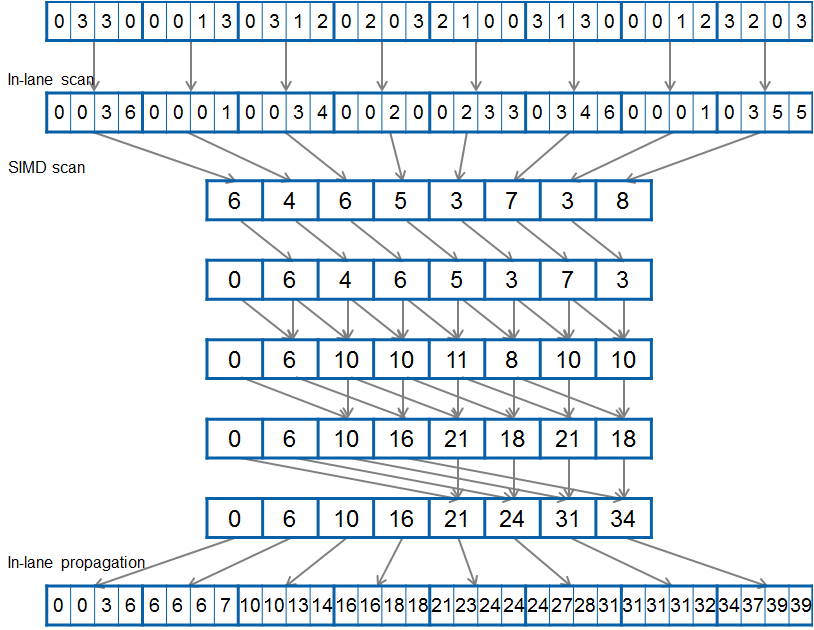
\includegraphics[width=\linewidth]{gpu-scan.png}
  \caption{\cite{harada2011introduction}}
  \label{fig:gpu-scan}
\end{figure}

Even if the prefix scan is computed efficiently, the scatter phase is still problematic. In the serialized version, after scanning the global digit counts, we copy the element to a second array at the position indicated by the counter for that digit, and we increment it. On the GPU this is problematic: it requires updating a value shared across blocks, and requires threads reading the same digit to maintain their relative order when copying. Harada-Howes \cite{harada2011introduction} illustrates a solution to this problem: instead of computing and scanning global digit counts, we compute block-privatized digit counts and scan them ordered, first by digit, then by block (the 0s of block 0, the 0s of block 1, ... the 1s of block 0, the 1s of block 1, ...). We obtain a sort of ``block-aware'' prefix sum as shown in \cref{fig:harada-howes-scan}.

\begin{figure}[htbp]
  \centering
  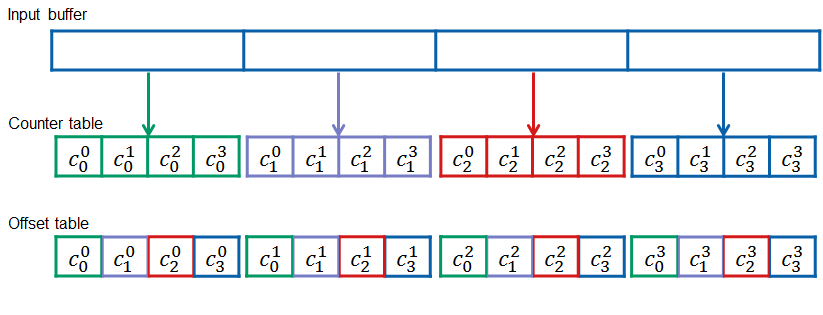
\includegraphics[width=\linewidth]{harada-howes-scan.png}
  \caption{\cite{harada2011introduction}}
  \label{fig:harada-howes-scan}
\end{figure}

With this, in the scatter phase each block knows the position at which it can start writing without interfering with other blocks.

All of the mentioned algorithms are radix sorts of the LSD variety (they iterate from LSD to MSD). However, the HRS algorithm \cite{10.1145/3035918.3064043}, which was the state of the art prior to \ones, is of the MSD variety (iterates from MSD to LSD), which was considered more performant. However, because \ones is an LSD radix sort, we will not delve into the MSD family.

\section{Onesweep}

To implement \ones, we followed the original paper by Adinets and Merril \cite{adinets2022onesweep}. The algorithm uses a number of parameters for each kernel which can be fine-tuned for the specific hardware, but we kept changes to a minimum, for a one-size-fits-all implementation. We leveraged templates to keep the algorithm very generic, on both the sorted type and the sorting key.

As radix, we followed the paper with \lstinline{RADIX=}256 and \lstinline{radix_size=}8bit. Moreover, in this project we used \lstinline{key_size=}32bit hash as key, thus \lstinline{digit_places=}4.

\subsection{Overview}

We give an overview of how the algorithm works and what each part aims to achieve. This way, later sections can focus on the ``how''s rather than the ``why''s.

The defining characteristic of \ones is that instead of doing a downsweep plus upsweep, it unifies the three phases in a single kernel that performs counting, prefix scan, and scattering. To achieve that, it preprocesses the input (``upfront phase'') to obtain the \emph{global} prefix scan of each digit place at once. As explained previously, this result is not directly useful for efficient parallel scattering, it is used instead to compute the final scatter offsets.

Then, we split the input into slices and iterate the sweep kernel for each digit place, one thread block per slice. Each block independently counts and computes a block-relative scatter offset for each element in the slice, along with the total count of each digit in the slice.

At this point the blocks collaborate with each other in a ``\emph{chained scan} with \emph{decoupled look-back}'' to compute the prefix sum of each digit's per block count. This result will be summed to the prefix sum of digit total counts (upfront phase), to obtain the starting scatter offset of each block's bins. Each digit's chained scan is performed in parallel by the first \lstinline{RADIX} threads of each block; this also dictates the minimum size of the block.

Finally, the computed upfront global prefixes, the result of the chained scan, and the block-relative offsets give each element's global scatter offset. However, in order to optimize memory coalescing, the elements are first scattered in shared memory (using the block-relative offset), then re-scattered in global memory using the global offset.

\subsubsection{Chained scan with decoupled look-back}

This is the main technique powering \ones. The idea is for each block to wait for the previous one to compute its prefix sum, but in a way that mitigates the latency.

On NVIDIA GPUs there's no fair scheduling (justice): when a SM is assigned a thread block, it will be run to completion before it can accept another (with the exception of context switching during long memory operations). This is sufficient to guarantee that when a block executes, the previous blocks are either still running or completed. There is still no guarantee on the order in which blocks are scheduled on the SMs, so the ``trick'' is to use a shared atomic counter in place of the built-in \lstinline{blockIdx} variable. Note that we do not have any guarantee on yet-to-be-run blocks, and waiting for them can easily result in deadlock; this also means we cannot wait for the entire chained scan to complete from inside a kernel.

The technique works by having each block atomically update a global array of counters and status flags. The array starts with all flags set to \lstinline{INVALID}. Each block \lstinline{i} produces its local count and atomically publishes it along with the status flag \lstinline{COUNT}. It then looks at the value published by \lstinline{i-1}:

\begin{itemize}
  \item If it's \lstinline{INVALID}, the block spin-waits for the value to change
  \item If it's \lstinline{PREFIX}, the block sums the value to its local count to obtain the prefix. It publishes it with the flag \lstinline{PREFIX} and moves on to the rest of the kernel
  \item If it's \lstinline{COUNT}, the block sums the value to its local count and looks at \lstinline{i-2}. The cycle repeats until it finds a \lstinline{PREFIX}
\end{itemize}

The one exception is the block \lstinline{0} that publishes \lstinline{PREFIX} immediately.

\begin{lstlisting}[caption={Pseudocode for Chained scan with decoupled look-back}, language=c]
int id = fetch_true_id()
int local_count = ...
Status local_status = COUNT

store(local_count, local_status);
  
for(i = id-1; local_status != PREFIX; --i) {
  StatusCount lookback;
  do {
    lookback = load(i)
  } while(lookback.status == INVALID);
  local_count += lookback.value
  local_status = lookback.status
}

store(local_count, local_status);
\end{lstlisting}

Each thread block needs to wait only for the blocks before it, and the furthest each block needs to look back is bound by (a small multiple of) the number of SMs. This makes full use of the parallel hardware and minimizes latency. Another intuition for this technique is running batches of $n$ blocks (where $n$ is the number of SMs) of a serial scan over $n$-wide slices, combining its lightness with efficient use of parallelization.

For the scheduling reasons mentioned before, having a block wait for the scan to complete (e.g. to access the total count) is not possible within the same kernel launch. Note that it would defeat the objective of this technique anyway (For completeness, it is technically possible to wait for the entire grid using cooperative groups; but in order to do that, the GPU needs enough shared memory and registers to accommodate the entire grid at once, which is unreasonable for our task).

\subsection{Upfront count}

The first step is to count the number of occurrences of each digit at each digit place, in the entire input array. Without any privatization. The kernel takes the data array and length, a \lstinline{u32[digit_places][radix]} table initialised to 0 to store the counts, and the hashing function.

The amount of threads per block is a static parameter (\lstinline{threads_per_block=}256) and so is the amount of blocks launched per SM (\lstinline{blocks_per_sm=}2). The length of the slices is determined by \lstinline{threads_per_block} times the static number of elements per thread (\lstinline{items_per_thread_per_slice=}8), giving a slice length of 2048 elements. The last slice may be smaller. If the actual number of slices in the data array results less than the capacity (i.e. \lstinline{blocks_per_sm} times the number of SMs), less blocks will be launched. 

Each block accesses the slices in \lstinline{gridDim} stride, while inside the block, threads access the elements in the slice in \lstinline{blockDim} stride. This way, consecutive blocks access consecutive slices, and consecutive threads in a block access consecutive elements in the slice. This is a common pattern used to optimize the usage of the L2 cache and memory coalescing. The slice length $>$1024 guarantees that slices are aligned to 1024 bytes no matter what the size of the data is, aligning the data to cache lines. However for efficient coalescing, the data elements must be of 1, 2, 4, 8, or 16 bytes. The data's type is templated and depends on the caller.

The kernel keeps a \lstinline{u32[digit_places][radix]} table of counters in shared memory. Once read and hashed an element, it iterates over its digit places and naively uses \lstinline{atomicAdd_block(&local_counts[place][digit], 1)} on the counter in shared memory. This is done without any kind of thread privatization or other contention reduction techniques to allow for a larger radix. Smaller radices lead to more digit places, and thus more iterations of the sorting kernel. The paper states that whatever the cost of this synchronization, it is completely recouped by the reduced iteration count. We must also keep in mind that on Maxwell architectures and later, atomic operations are handled by native hardware units in the memory controller, and much cheaper than they used to be.

\begin{lstlisting}[caption={Local counting phase}, language=c++]
// iterate over slices in strides of grid size
for (u32 i = blockIdx.x * slice_length; i < length; i += gridDim.x * slice_length) {
  // iterate over the data slice in strides of block size
  u32 const slice_end = min(length, i + slice_length);
  for (u32 j = i + threadIdx.x; j < slice_end; j += blockDim.x) {
    Data const item = data[j];
    typename Key::KeyType const hash = hasher(item);
    // for each digit place in the key
    for (u8 place = 0; place < Key::digit_places; ++place) {
      // extract digit
      u16 const digit = Key::extract_digit(hash, place);
      // increment corresponding counter
      atomicAdd_block(&local_counters[place][digit], 1);
    }
  }
}
\end{lstlisting}

\newpage

After iterating through the entire data array, each block \lstinline{atomicAdd}s the local counter table to the one in global memory. The threads access the table in a linearized way to allow for memory coalescing.

\begin{minipage}{\dimexpr\linewidth-15pt\relax} %avoids breaking the code in two pages
\begin{lstlisting}[caption={Updating the global count}, language=c++]
// cast the arrays as a flat 1D layout
auto const linearized_global_counters = flatten(counters);
// parallel write to global memory
for (u16 i = static_cast<u16>(threadIdx.x); i < cuda::std::size(linearized_global_counters); i += blockDim.x) {
  u32 const count = linearized_local_counters[i];
  if (count) {
    atomicAdd(&(linearized_global_counters)[i], count);
  }
}
\end{lstlisting}
\end{minipage}

At this point one might wonder why not go beyond an 8bit radix. With 64bit keys, we would need at least a 10bit radix to shave off one iteration, all the way to 11 bits for 32bit keys. This makes radices between 256 and 1024 effectively useless, and while a radix of 1024 might still be feasible for this upfront count kernel, it's likely too large for the sweep kernel.

\subsection{Upfront prefix scan}

The next step is to compute the prefix sum of the just-computed upfront count. The same block-local and warp-local prefix sum routines described here will also be used by the sweep kernel. The code reflects both use cases.

As an optimisation, this kernel detects if a digit place is ``degenerate'', meaning that all input elements share the same digit. If that is the case, we can skip launching the sweep kernel for that place. It is quite cheap to detect and especially effective in the case of hashes that are bound in some way by the length of the data (modulo in our use case).

We perform the prefix sum by launching \lstinline{digit_places} blocks of \lstinline{RADIX} threads. Each block is assigned to one of the digit places, and performs the prefix sum of the counters of each digit. The high level code of the kernel is fairly simple, it leans entirely on the \lstinline{radix_scan} function we will discuss later, and only handles reading and writing from global memory.

\begin{minipage}{\dimexpr\linewidth-15pt\relax} %avoids breaking the code in two pages
\begin{lstlisting}[caption={Upfront prefix sum kernel}, language=c++]
template <IsInstanceOf<Key> Key> KERNEL void exclusive_scan(Counters<Key> *const counters, u32 const length) {
  auto const result = radix_scan<true>((counters->counters)[blockIdx.x][threadIdx.x], length);
  if (threadIdx.x == 0) {
    (counters->degenerates)[blockIdx.x] = !result.has_value();
  }
  if (result) {
    (counters->counters)[blockIdx.x][threadIdx.x] = *result;
  }
}
\end{lstlisting}
\end{minipage}

\subsubsection{Parallel prefix sum algorithms and GPUs}

In literature there are two classical parallel prefix sum algorithms: a latency-efficient one (Hillis-Steele \cite{10.1145/7902.7903}), and a work-efficient one (Blelloch \cite{42122}). The former minimizes the height of the compute graph, at the expense of the total number of operations; the latter minimizes the number of total operations, at the expense of the height of the compute graph. Usually, latency-efficient algorithms are preferred when the number of processors matches the length of the input.

For this reason, GPU Gems 3 \cite{nguyen2007gpu} recommends Blelloch's algorithm. Back then, streaming multiprocessors where extremely small by today's standards, a Tesla GPU had only $\sfrac1 4$ warp per SM (8 cores), and the later Fermi GPUs had two $\sfrac1 2$ warps (16+16 cores). Both algorithms also made heavy use of shared memory and \lstinline{__syncthreads()} for thread cooperation, so a work-efficient approach was a given. On modern hardware however, SMs are much less ``core-starved'', and most importantly, warp level intrinsics make Hillis-Steele extremely efficient and thus the better choice for short arrays like our case. Note that we're talking about block-level scans, in multi-block scenarios both algorithms become impractical, and more complex approaches (e.g. chained scan) become necessary.

To maximise the use of warp-level intrinsics, we subdivide into sub-scans as usual, this time warp sized.

\subsubsection{Warp-level prefix sum}

The Hillis-Steele parallel prefix sum starts by assigning an element to each thread, with value $k$ set to 1. At each iteration, all threads with $id>k$ sum their value to the one of $id-k$. $k$ is doubled at each iteration, therefore we iterate $\log_{2}(n)$ times. Unlike Blelloch, the algorithm can be implemented to work even if $n$ is not a power of two; in our case it wasn't important so we decided to keep our implementation fast and simple.

\begin{figure}[h]
    \centering
    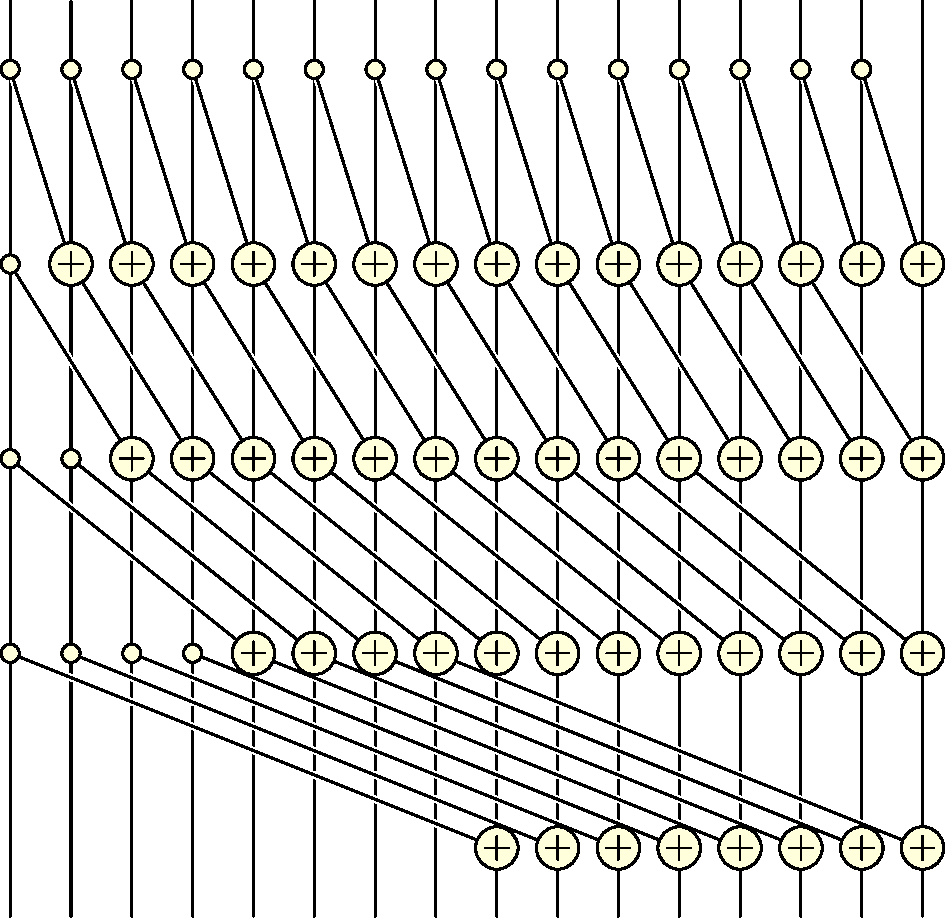
\includegraphics[scale=0.42]{Hillis-Steele_Prefix_Sum.pdf}
    \caption{Diagram \cite{wiki:prefix_sum} of Hillis-Steele prefix sum}
    \label{fig:hillis-steele}
\end{figure}

We implement a warp-level Hillis-Steele prefix sum using the \lstinline{__shfl*_sync} family warp intrinsic, which allows threads to ``send'' a value to other threads in the warp, whilst receiving themselves a value that was sent to them. This is conceptually similar to storing a value in a warp-privatized shared memory array then synchronizing the warp, but it's implemented in hardware and much more efficient; the shared memory load/store is skipped entirely and without needing a true thread fence.

In particular we use \lstinline{__shfl_up_sync(mask, value, offset, width)}, that receives \lstinline{value} from the thread \lstinline{lane}-\lstinline{offset}, partitioning the operation in ``chunks'' of \lstinline{width} lanes. The mask indicates which lanes participate in this shuffle operation, and requires caution to avoid deadlocks and undefined behaviours. There are also some discrepancies between what works on pre and post Volta architectures, with post-Volta being more flexible but more prone to deadlocks. With our main targets being Turing and Pascal, we took care to write correct code for both architectures.

\begin{lstlisting}[caption={Warp-level inclusive prefix sum}, language=c++]
// intra-warp inclusive prefix sum using register shuffles
template <u8 width = 32, std::integral Data>
GPU inline Data warp_inclusive_multiscan(Data val, u32 const thread_mask = SYNC_WARP) {
  static_assert(cuda::std::has_single_bit(width), "Width of warp_inclusive_scan must be a power of two");
  static_assert(width <= 32, "Width of warp_inclusive_scan must <= 32");
#pragma unroll
  for (u32 offset = 1; offset < width; offset <<= 1) {
    Data const remote_val = __shfl_up_sync(thread_mask, val, offset, width);
    if ((threadIdx.x % width) >= offset) {
      val += remote_val;
    }
  }
  return val;
}
\end{lstlisting}

This function is templated on the width of the scan, but it is implemented so that, with an appropriate \lstinline{thread_mask}, a single warp can perform multiple smaller scans.

Note that the function implements an \emph{inclusive} prefix sum, because the exclusive sum is obtained by performing an extra \lstinline{__shfl_up_sync(mask, value, 1, width)}.

\enlargethispage{1\baselineskip}

\subsubsection{Block-level prefix sum}

The general outline of the block level prefix sum is:
\begin{enumerate}
  \item Each warp computes a warp-level inclusive sum
  \item One thread per warp publishes the total sum to a shared memory array
  \item One warp computes the warp-level inclusive sum of the published totals
  \item Each warp converts its inclusive sum into an exclusive sum
  \item Each warp sums the appropriate prefixed total to its prefixed elements
\end{enumerate}

\begin{minipage}{\dimexpr\linewidth-15pt\relax} %avoids breaking the code in two pages
\begin{lstlisting}[caption={block-level exclusive sum, stripped of degeneracy detection}, language=c++]
GPU inline u32 radix_scan(u32 const digit_count) {
  // threads must be within the radix range
  assert(threadIdx.x < RADIX);

  constexpr u8 warps = RADIX / 32;
  u8 const lane = threadIdx.x % 32;
  u8 const warp_id = static_cast<u8>(threadIdx.x / 32);

  // shared memory to store the aggregate sum of each warp
  SHARED u32 warp_counters[warps];
  SHARED std::conditional_t<detect, u32[warps], char> degenerate_warps;


  u32 sum = warp_inclusive_multiscan(digit_count);

  // last thread in each warp publishes the warp total
  if (lane == 31)
    warp_counters[warp_id] = sum;

  __syncthreads();

  // warp 0 scans the warp totals
  if (warp_id == 0) {
    u32 const sum = warp_inclusive_multiscan<warps>((lane < warps) ? warp_counters[lane] : 0);
    if (lane < warps)
      warp_counters[lane] = sum;
  }

  __syncthreads();

  sum = __shfl_up_sync(SYNC_WARP, sum, 1);
  if (lane == 0)
    sum = 0;

  // add prefix sum of previous warps to local warp results
  if (warp_id > 0)
    sum += warp_counters[warp_id - 1];

  return sum;
}
\end{lstlisting}
\end{minipage}

In this function the length of the scan is hardcoded to exactly \lstinline{RADIX} elements (unlike \lstinline{warp_inclusive_multiscan}) to reduce code complexity. The \lstinline{RADIX} is still parametric, and the function supports radices up to 1024, i.e. until \lstinline{warps} is $\leq$32.

By using a templated boolean \lstinline{detect} paired with \lstinline{if constexpr}, we can toggle detection of degenerate digit places at compile time, at zero cost. The upfront prefix scan kernel uses this function with detection enabled, so if the returned optional is \lstinline{nullopt}, the first thread will publish \lstinline{true} on the array of degenerate places. We call a digit place's counts degenerate if there is a digit where \lstinline{digit_count == length}. That implies all other counts to be 0 and we avoid a useless sorting pass.

\begin{minipage}{\dimexpr\linewidth-15pt\relax} %avoids breaking the code in two pages
\begin{lstlisting}[caption={Degeneracy detection, stripped of the prefix sum}, language=c++]
template <bool detect = false>
GPU inline std::conditional_t<detect, cuda::std::optional<u32>, u32>
radix_scan(u32 const digit_count, std::conditional_t<detect, u32, std::monostate> const length = std::monostate{}) {
  //////// init ////////

  // scan within each warp
  bool degenerate_warp;
  if constexpr (detect) {
    // detect if the warp is degenerate, i.e. only one digit population
    degenerate_warp = __any_sync(SYNC_WARP, digit_count == length);
  }

  //////// per warp sum ////////

  if (lane == 31)
    if constexpr (detect) 
      degenerate_warps[warp_id] = degenerate_warp;

  __syncthreads();

  SHARED bool degenerate_block;

  // warp 0 scans the warp totals
  if (warp_id == 0) {
    bool flag = false;
    if constexpr (detect) {
      flag = __any_sync(SYNC_WARP, (lane < warps) ? degenerate_warps[lane] : 0);
      if (lane == 0)
        degenerate_block = flag;
    }
    if (!flag) 
      //////// sum of warp totals ////////
  }

  __syncthreads();

  if constexpr (detect) {
    if (degenerate_block)
      return cuda::std::nullopt;
  }

  //////// conclusion ////////
}
\end{lstlisting}
\end{minipage}

With the global prefix scan computed and the degenerate places detected, the upfront part of the algorithm is completed. Before moving to the sweep part, it's useful to go back to the upfront scan kernel equipped with a better understanding of \lstinline{radix_scan}. It's also important to get familiar with how \lstinline{warp_inclusive_multiscan} can compute multiple smaller prefix scans at once, as this feature will be used in the sweep phase.

\subsection{Sweep kernel}

This is the core part of the sorting algorithm. The sweep kernel is iterated for all non-degenerate digit places, each times it reads an array, and copies it partially sorted on a second array. After at most \lstinline{RADIX} iterations, the array is sorted. The kernel is launched with a static number of threads per block (\lstinline{threads_per_block=}256), and as many blocks as there are slices. Each thread processes a static amount of items (\lstinline{items_per_thread=}8), resulting in a slice length of (the last slice might be shorter). These parameters could be fine-tuned, like the parameters of the upfront count phase. The parameters for the two phases don't need to match.
The paper was able to process between 21 and 46 items per thread due to a much larger shared memory than our test hardware.

We can split this kernel into three phases plus an initialisation one. The initialisation phase only needs to obtain the ``actual'' block id, initialise a shared memory array, and calculate some constants that will be used by the algorithm. The other three phases are:

\begin{enumerate}
  \item Computing block-relative prefix sums for each digit
  \item Chained scan of the total counts per digit
  \item Scattering, first in shared memory, then global
\end{enumerate}

As explained before, the chained scan relies on the fact that each block can assume all blocks that started running before it are either still running or complete. But the GPU makes no guarantees on the order in which blocks are scheduled, so we need to obtain an id that actually reflects the order in which blocks are being executed. This is done using an atomic counter.

\begin{lstlisting}[caption={Initialisation phase of the sweep kernel}, language=c++]
inline constexpr u16 slice_max_length = threads_per_block * items_per_thread;
inline constexpr u8 warp_slices = threads_per_block / 32;
static_assert(warp_slices <= 32, "warp_slices must be at most 32");
inline constexpr u16 warp_slice_max_length = 32 * items_per_thread;
inline constexpr u8 subwarp_size = pow2_ceiling(warp_slices);
inline constexpr u8 subwarps_per_warp = 32 / subwarp_size;
inline constexpr u16 subwarps = warp_slices * subwarps_per_warp;

template <typename Data, is_hasher<Data> Hasher>
KERNEL void onesweep(u32 *const atomic_id,
                     Data const *const data,
                     Data *const sorted,
                     u32 const length,
                     u8 const place,
                     StateCounter *const linearized_global_state_counters,
                     u32 const (&global_totals)[RADIX],
                     Hasher const hasher) {
  using Key = Key<Data, Hasher>;
  SHARED u32 block_id; // NOLINT(bugprone-dynamic-static-initializers)
  if (threadIdx.x == 0) {
    block_id = atomicAdd(atomic_id, 1) % gridDim.x;
  }

  // RADIX is multiple of 32, thus row reads are guaranteed to conflict
  // RADIX + subwarps_per_warp offsets the rows by subwarp slice
  SHARED u16 slice_prefixes[warp_slices][RADIX + subwarps_per_warp];
  auto const linearized_slice_prefixes = flatten(slice_prefixes);
  for (u16 i = static_cast<u16>(threadIdx.x); i < static_cast<u16>(cuda::std::size(linearized_slice_prefixes));
       i += blockDim.x) {
    linearized_slice_prefixes[i] = 0;
  }

  __syncthreads();

  u8 const lane = threadIdx.x % 32;
  u16 const warp_id = static_cast<u16>(threadIdx.x) / 32;
  u16 const subwarp_id = static_cast<u16>(threadIdx.x) / subwarp_size;
  u8 const subwarp_lane = threadIdx.x % subwarp_size;
  u32 const slice_start = block_id * slice_max_length;
  u32 const slice_end = min(length, slice_start + slice_max_length);
  u16 const slice_length = static_cast<u16>(slice_end - slice_start);
  u32 const warp_slice_start = min(slice_end, slice_start + warp_id * warp_slice_max_length);
  u32 const warp_slice_end = min(slice_end, warp_slice_start + warp_slice_max_length);
  u16 const warp_slice_length = static_cast<u16>(warp_slice_end - warp_slice_start);

  u16 warp_slice_prefix[items_per_thread];
\end{lstlisting}

\subsubsection{Block-relative prefix sums}

This is arguably the most byzantine part of the algorithm. We divide the input slice further into \lstinline{warp_slices=threads_per_block/32} sub-slices of \lstinline{warp_slice_length=32*items_per_thread} elements (the last sub-slice might be shorter). Let's ignore sub-slices and global scattering for now and assume we only need to sort a block slice. To scatter the elements we need a per-digit prefix sum of warp-privatized digit counts. We also need a per-digit digit-privatized prefix sum (in other words, each thread needs to know its position among the others holding the same digit, within the warp).

Each of these values has a specific meaning:

\begin{itemize}
  \item Prefix sum of block-privatized digit counts: starting offset of the digit bins
  \item Per-digit prefix sum of warp-privatized (block-relative) digit counts: starting offset of the warp \emph{in} each digit's bin
  \item Per-digit prefix sum of digit-privatized (warp-relative) counts: offset of each item from the starting offset of the warp
\end{itemize}

\newpage
\enlargethispage{1\baselineskip}

Putting them together, given an item, we sum: the offset of its digit bin in the block, the offset of the warp in the digit bin, and the offset of the item in the warp; which gives us the final scatter position of the item in shared memory. Stepping back, to get the global scatter position we just swap the first component with its global counterpart: the global prefix sum computed upfront (starting offset of the digit bin) plus the digit-relative offset of the block, given by the chained scan.

To implement this, we keep an \lstinline{u16 slice_prefixes[warp_slices][RADIX]} array where each warp counts the digits in its warp slice. We then compute \lstinline{RADIX} prefixes sums, one for each digit, summing over the warp counts for each digit. If the number of warps is less than 32 (8 in our parameters), a single warp can perform multiple sums at once (4 in our case) in batches we call ``subwarps''. We previously discussed this mode of operation of \lstinline{warp_inclusive_multiscan}. One additional quirk comes from the fact that warps access \lstinline{slice_prefixes} column major, \lstinline{subwarps_per_warp} columns per iteration, and a matrix row is a multiple of the warp delivery capacity 32$\times$4bytes. This guarantees bank conflicts, as each warp accesses column-aligned row slices. Our solution is to map each row access to a different bank column by introducing padding so that slices become staggered. Thus we get \lstinline{u16[warp_slices][RADIX+subwarps_per_warp]}. Note that using \lstinline{u16} instead of \lstinline{u32} means that pairs of columns are stored on the same bank.

\begin{figure}[htbp]
  \centering
  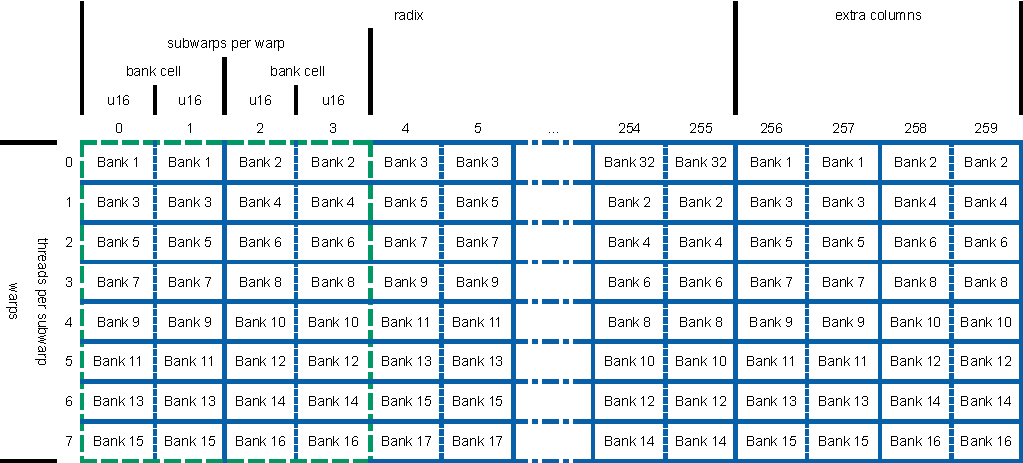
\includegraphics[width=\linewidth]{yipe-matrix-alignment.pdf}
  \caption{Layout of the matrix and access pattern}
  \label{fig:matri-alignement}
\end{figure}

\begin{figure}[htbp]
  \centering
  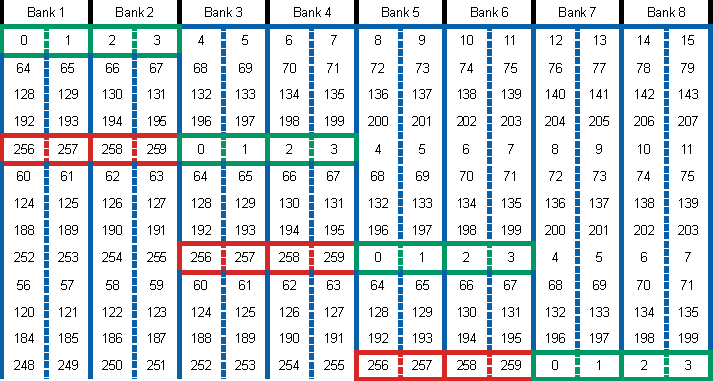
\includegraphics[width=\linewidth]{yipe-bank-alignment.pdf}
  \caption{Layout of the matrix in the first 8 memory banks}
  \label{fig:bank-alignment}
\end{figure}

Because these are \emph{inclusive} prefix sums, the last line of the array contains the block-wide counts of each digit; this will later be used to compute the prefix sum of block-privatized digit counts to participate in the chained scan.

At each iteration we use the \lstinline{__match_any_sync} warp intrinsic to get a bitmask of the lanes with the same digit, and only one leader per digit updates the count. We use the \lstinline{__popc} bit-op intrinsic to count the 1s in the mask. The leader also ``sends'' the previous count to the lanes with the same digit using a \lstinline{__shfl_sync} warp intrinsic. Each lane uses the bitmask and the value read from the leader to compute the warp-slice-relative prefix sum of its item, and stores it in a private array. In the scatter phase, each thread re-reads the exact same items in the exact same order, keeping the association between prefix and item. We took care to make sure the array does not spill in local memory, and resides entirely in the registers.

\begin{lstlisting}[caption={Block-relative prefix sums}, language=c++]
// iterate over the data slice, partitioned by warps
// iterate over `pass` with explicit bound instead of `i`
// prevents spilling of `warp_slice_prefix`
for (u16 pass = 0; pass < items_per_thread && pass * 32 + lane < warp_slice_length; ++pass) {
  u32 i = pass * 32 + lane;
  u8 const warp_usage = static_cast<u8>(min(warp_slice_length - pass * 32, 32U));
  u32 const thread_mask = __funnelshift_lc(UINT_MAX, 0, warp_usage);
  Data const item = data[warp_slice_start + i];
  typename Key::KeyType const hash = hasher(item);
  u16 const digit = Key::extract_digit(hash, place);
  u32 const matches = match_any_polyfill<RADIX_SIZE>(digit, thread_mask);
  // __ffs is 1-indexed
  u8 const leader_id = __ffs(matches) - 1;

  u16 prefix = 0;

  if (lane == leader_id) {
    prefix = slice_prefixes[warp_id][digit];
    slice_prefixes[warp_id][digit] += __popc(matches);
  }
  __syncwarp(thread_mask);

  // share the exclusive sum within the warp
  prefix = __shfl_sync(thread_mask, prefix, leader_id);
  // each thread sums its own prefix
  // warp_slice-relative counts are stored in shared memory
  warp_slice_prefix[pass] = prefix + __popc(matches & (1u << lane) - 1);
}

__syncthreads();(*@\newpage@*)
// iterate over the warp_slice counters of each digit
for (u16 i = subwarp_id; i < RADIX; i += subwarps) {
  u16 val = subwarp_lane < warp_slices ? slice_prefixes[subwarp_lane][i] : 0;
  val = warp_inclusive_multiscan<subwarp_size>(val);
  if (subwarp_lane < warp_slices) {
    slice_prefixes[subwarp_lane][i] = val;
  }
}
\end{lstlisting}

Pre-Volta GPUs do not support \lstinline{__match_any_sync}. We wrote a wrapper \lstinline{match_any_polyfill} that uses the intrinsic if present, and emulates it (polyfilling) otherwise, using the \lstinline{__ballot_sync} warp intrinsic and bit operations. The paper doesn't mention the \lstinline{__match_any_sync} intrinsic, but describes the emulation process.

\begin{lstlisting}[caption={\lstinline{\_\_match\_any} with polyfilling}, language=c++]
template <u8 size> GPU u32 match_any_polyfill(u16 const key, u32 const thread_mask = SYNC_WARP) {
#if __CUDA_ARCH__ >= 700
  // sm_70+ volta, turing, ...
  return __match_any_sync(thread_mask, key);
#else
  CPRINT("match_any polyfilled (__CUDA_ARCH__=" XSTR(__CUDA_ARCH__) ")")
  u32 candidates = thread_mask;
  for (u16 mask = 1; mask < 1 << size; mask <<= 1) {
    u16 bit = key & mask;
    candidates &= __ballot_sync(thread_mask, static_cast<int>(bit)) ^ (UINT_MAX * !bit);
  }
  return candidates;
#endif
}
\end{lstlisting}

\subsubsection{Chained scan}

After the block-relative \emph{inclusive} prefix sums have been computed, the last row of \lstinline{slice_prefixes} contains the block-privatized count of each digit, necessary for the block to participate in \lstinline{RADIX} chained scans. The result will be the digit-relative offset of the block. We already went over the ideas behind it, so now we'll focus on the code.

The first challenge is to keep the status flags and the published values consistent. Following the paper, we store both in the same 32bit word; 2 bits for the flag and 30 bits for the value. Since these are digit counts, the algorithm won't work if there are $\geq2^{30}$ occurrences of the same digit (in a non-degenerate digit place). If the architecture supports larger atomic operations, this limit can be raised to $2^{62}$, or even $2^{126}$, although this is taxing on performance. We are targeting architectures as low as Pascal, which supports up to 64bit atomics, however, in our case we don't need more than 32 bits. We implement this with bitfields.

\newpage

\begin{lstlisting}[caption={Status + counter bitfield}, language=c++]
enum class State : u32 {
  Invalid = 0,
  Count = 1,
  Prefix = 2,
};

struct StateCounter {
  State status : 2;
  u32 counter : 30;
};
\end{lstlisting}

We note that in the paper, statuses and counters are stored in a \lstinline{StatusCounter[RADIX][slices]} array, and not the other way around. This layout favours iterating over the blocks rather than memory coalescing. We use \lstinline{cuda::atomic_ref} for the atomic operation, and \lstinline{cuda::std::span} or \lstinline{cuda::std::mdspan} to make array access safer and simpler. For each digit the chained scan is performed by the first \lstinline{RADIX} threads of each block, and the results are stored in \lstinline{global_prefix}.

By keeping the block-privatized totals separate from the chained scan ones, we can hold off computing their prefix sum until after the scan. This lets us publish as soon as possible without yet another array in shared memory.

\begin{lstlisting}[caption={Chained scan}, language=c++]
// chained scan exclusive sums
SHARED u32 global_prefix[RADIX];
cuda::std::span const slice_totals(slice_prefixes[warp_slices - 1], RADIX);

if (threadIdx.x < RADIX) {
  // slice containing the slice totals
  using global_state_counters_extents = cuda::std::extents<u32, RADIX, cuda::std::dynamic_extent>;
  cuda::std::mdspan<StateCounter, global_state_counters_extents> const global_state_counters(
      linearized_global_state_counters, global_state_counters_extents{gridDim.x});
  // fenced global memory state_counter
  cuda::atomic_ref<StateCounter, cuda::thread_scope_device> const global_state_counter(
      global_state_counters(threadIdx.x, block_id));

  // publish the block totals
  global_state_counter.store({block_id == 0 ? State::Prefix : State::Count, slice_totals[threadIdx.x]},
                             cuda::memory_order_release);(*@\newpage@*)

  global_prefix[threadIdx.x] = 0;
  for (u32 i = block_id - 1; block_id != 0; --i) {
    cuda::atomic_ref<StateCounter, cuda::thread_scope_device> const sc_ref(global_state_counters(threadIdx.x, i));
    StateCounter sc = sc_ref.load(cuda::memory_order_acquire);
    while (sc.status == State::Invalid) {
      nanosleep_polyfill(32);
      sc = sc_ref.load(cuda::memory_order_acquire);
    }

    global_prefix[threadIdx.x] += sc.counter;
    if (sc.status == State::Prefix) {
      // publish the total inclusive prefix
      global_state_counter.store({State::Prefix, global_prefix[threadIdx.x] + slice_totals[threadIdx.x]},
                                 cuda::memory_order_release);
      break;
    }
  }

  // scan the block totals
  slice_totals[threadIdx.x] = static_cast<u16>(radix_scan(slice_totals[threadIdx.x]));
}
\end{lstlisting}

In the spin-wait we use \lstinline{__nanosleep} as a yielding operation. Pascal doesn't support \lstinline{__nanosleep} and doesn't have an equivalent, so \lstinline{nanosleep_polyfill} simply does nothing on pre-Volta architectures.

The last step is computing the aforementioned exclusive prefix sum of the block-privatized digit counts. We now have all the information we need to perform the scattering.

\subsubsection{Scattering}

This last phase consists in putting together the offsets we have computed. As mentioned before, to help with memory coalescing, the data is scattered in shared memory first, then the digit bins are copied to global memory.

Some of the components necessary to compute the scatter offsets are warp-local or thread-local. When the shared memory bins are copied to global memory, these components become inaccessible because the order of the items has changed, and cannot be traced back.
We can still extract them from each item's shared memory index by subtracting the block-relative bin offset for that digit.

For the local scatter phase, we re-read the items from global memory. We could've store them in shared memory when they are read at the beginning of the kernel, but the item type is generic, and its size is bound by the scatter array. Adding a second array would halve the maximum item size.
The GPU may still avoid double global memory access as it automatically utilises the leftover shared memory as L1 cache. This way the algorithm still works with large items, just slower.

\newpage

\begin{lstlisting}[caption={Scattering}, language=c++]
  SHARED Data bins[slice_max_length];

  // iterate over the data slice, partitioned by warps
  // iterate over `pass` with explicit bound instead of `i`
  // prevents spilling of `warp_slice_prefix`
  for (u16 pass = 0; pass < items_per_thread && pass * 32 + lane < warp_slice_length; ++pass) {
    u32 i = pass * 32 + lane;

    Data const item = data[warp_slice_start + i];
    typename Key::KeyType const hash = hasher(item);
    u16 const digit = Key::extract_digit(hash, place);

    u16 const dest =
        slice_totals[digit] + (warp_id == 0 ? 0 : slice_prefixes[warp_id - 1][digit]) + warp_slice_prefix[pass];
    bins[dest] = item;
  }

  __syncthreads();

  for (u16 i = static_cast<u16>(threadIdx.x); i < slice_length; i += blockDim.x) {
    Data const item = bins[i];
    typename Key::KeyType const hash = hasher(item);
    u16 const digit = Key::extract_digit(hash, place);

    u32 const global_dest = global_totals[digit] + global_prefix[digit] + i - slice_totals[digit];
    sorted[global_dest] = item;
  }
}
\end{lstlisting}

\chapter{Spatial hash table}

\section{Spatial hashing}

A spatial hash is a hashing function that preserves some form of spatial information, typically used on coordinates; their primary purpose is to speed up space related queries.
Usually, spatial hash functions are designed so that if point $b$ is within a certain radius of point $a$, it's possible to infer the hash of $b$ and directly look up its bucket. It may be required to iterate a number of buckets until $b$ is found, depending on the radius and the coordinate space's size.

Generally, spatial hash functions discretise the coordinates by dividing them by the radius with truncation. The discretised coordinates now identify a cell in a discrete space, where we apply a standard hashing function.

A spatial hash function can have collisions, where multiple cells map to the same bucket, or it can be a perfect spatial hash function, where each cell is mapped to its own bucket. A perfect hash function can lead to faster queries, but requires a hash table that is as large as the total number of buckets. We use a regular non-perfect function.

When we only query over a specific radius, the size of the discrete cells should be the same as the radius, to minimise both the number of buckets to examine and the number of outside points in those buckets.
Querying an arbitrary 3D point requires examining 27 buckets while in the discrete space it only requires 8.

The kernels take a closure defined as the struct \lstinline{PointHasher}, which can be built from a radius and a particle count using \lstinline{get_hasher}. We also define an \lstinline{is_hasher} concept, to be used in templates.

\begin{lstlisting}[caption={Spatial hash function}, language=c++]
template <typename Func, typename T>
concept is_hasher = requires(Func const f, T const val) {
  // enforces that f(val) is valid and returns an unsigned integer
  { f(val) } -> std::unsigned_integral;
};

GPU HOST inline u32 point_hash_inline(u323 const discrete, u32 const particle_count) {
  static u32 const primes[3] = {73856093, 19349663, 83492791};
  return ((discrete.x * primes[0]) ^ (discrete.y * primes[1]) ^ (discrete.z * primes[2])) % particle_count;
}(*@\newpage@*)
GPU HOST inline u32 point_hash_inline(float4 const point, u32 const particle_count, float const particle_radius) {
  return point_hash_inline({static_cast<u32>(point.x / particle_radius),
                            static_cast<u32>(point.y / particle_radius),
                            static_cast<u32>(point.z / particle_radius)},
                           particle_count);
}

struct PointHasher {
  u32 length;
  float particle_radius;

  GPU HOST inline u32 operator()(float4 const p) const { return point_hash_inline(p, length, particle_radius); }
  GPU HOST inline u32 operator()(u323 const cell) const { return point_hash_inline(cell, length); }
};

GPU HOST inline PointHasher get_hasher(u32 const length, float const particle_radius) noexcept {
  return PointHasher{length, particle_radius};
}
\end{lstlisting}

Note that the hasher can either discretise and hash continuous coordinates, or hash already discretised coordinates. This is done to avoid the numerical instability of converting from discrete to continuous to discrete again. In our case this manifested as artifacts of the isosurfaces. 

\enlargethispage{1\baselineskip}

\section{Parallelised hash table}

The idea behind a parallelised hash table is simple but presents some implementation pitfalls. The idea is to first sort the data by hash, then look for positions where \lstinline{hash(data[i]) != hash(data[i+1])} (in parallel). Those positions are the bucket boundaries, so it's just a matter of keeping a table with one place per bucket.
Using two arrays, or an array of pairs, to store both the beginning and end of each bucket would waste memory, since a bucket ends where the next one begins.

Now, if the bucket $b+1$ is not present in the table, we don't know where bucket $b$ ends. To solve this, when we find a boundary between \lstinline{i} and \lstinline{i+1}, we need to both record the beginning of the bucket at \lstinline{i+1}, and the end of the bucket at \lstinline{i}. If we notice that the buckets at \lstinline{i} and \lstinline{i+1} are consecutive, then we skip writing the end of \lstinline{i} because it is the beginning of \lstinline{i+1}.

We need to detect when a bucket is missing: intuitively this occurs when its start or end position are missing, but we still need a \emph{value} to represent an empty position. We free up the 0 value by adding 1 to each stored position (limiting by one the maximum data size), then at lookup we check for 0 or subtract 1. Another option is to use a bitfield, which halves the maximum size.

We store the table in an open-ended struct describing its size. We add an extra cell at the end to account for the end of the last bucket, simplifying the lookup logic.

\begin{lstlisting}[caption={Hash table structure}, language=c++]
struct Bucket {
  u32 begin, end;
};

struct HashTable {
  u32 length; // number of buckets + 1
  u32 table[1];

  template <std::unsigned_integral Hash> GPU cuda::std::optional<Bucket> lookup(const Hash hash) const {
    assert(hash + 1 < this->length);
    const u32 begin = this->table[hash];
    const u32 end = this->table[hash + 1];

    if (begin == 0 || end == 0 || begin == end) {
      return cuda::std::nullopt;
    }

    return Bucket{begin - 1, end - 1};
  }
};
\end{lstlisting}

The kernel that builds the hash table iterates similarly to the upfront count kernel, with additional edge cases at the slice boundaries.

\newpage

\begin{lstlisting}[caption={Hash table building kernel}, language=c++]
template <typename Data, is_hasher<Data> Hasher>
KERNEL void
build(Data const *const data, u32 const length, HashTable *const hash_table, u32 const buckets, Hasher const hasher) {
  using Key = Key<Data, Hasher>;
  hash_table->length = buckets + 1;
  cuda::std::span<u32, cuda::std::dynamic_extent> table(hash_table->table, buckets + 1);
  assert(length > 0);

  for (u32 i = blockIdx.x * slice_length; i < length; i += gridDim.x * slice_length) {
    // iterate over the data slice in strides of block size
    // if first element[0], add manually.
    u32 const loop_start = i + threadIdx.x;
    if (loop_start == 0) {
      Data const item = data[0];
      typename Key::KeyType const hash = hasher(item);
      table[hash] = 1;
    }
    // check the slice fits inside length-1, we are reading two points at a time
    u32 const slice_end = min(length - 1, i + slice_length);
    u32 j;
    for (j = loop_start; j < slice_end; j += blockDim.x) {
      Data const item_left = data[j];
      typename Key::KeyType const hash_left = hasher(item_left);
      assert(hash_left < buckets); // invalid hash function
      Data const item_right = data[j + 1];
      typename Key::KeyType const hash_right = hasher(item_right);
      assert(hash_right < buckets);    // invalid hash function
      assert(hash_left <= hash_right); // unsorted data

      if (hash_left != hash_right) {
        // next hash after left
        u32 const left_next = hash_left + 1;
        // end of the left bucket (+1)
        u32 const left_end = j + 2;

        // publish end of left bucket
        table[left_next] = left_end;
        // if the right bucket *is* left_next, nothing to do
        if (hash_right > left_next) {
          // the start of the right bucket is the end of the left bucket
          table[hash_right] = left_end;
        }
      }
    }
    if (j == length - 1) {
      Data const item = data[j];
      typename Key::KeyType const hash = hasher(item);
      table[hash + 1] = length + 1;
    }
  }
}
\end{lstlisting}

\chapter{Standalone prefix scan}

To implement marching cubes we require a prefix sum algorithm to pre-calculate the geometry buffer size. We implemented one following the same chained scan technique from \ones. By stripping the rest of the sorting algorithm, we get a kernel that can handle larger batches. We use blocks of \lstinline{threads_per_block=}512 threads that process \lstinline{items_per_thread=}12 items per thread, for a slice size of \lstinline{warp_slice_length=threads_per_block*items_per_thread} elements.

The block-relative prefix sum mirrors the initial block-relative prefix sums of \ones, but is greatly simplified, as there are no digits to match and count separately. 

\enlargethispage{2\baselineskip}

\begin{lstlisting}[caption={Block-relative prefix sum}, language=c++]
  SHARED Data slice_prefixes[warp_slices];
  for (u16 i = static_cast<u16>(threadIdx.x); i < cuda::std::size(slice_prefixes); i += blockDim.x) {
    slice_prefixes[i] = 0;
  }

  __syncthreads();


  Data warp_slice_prefix[items_per_thread];

  // iterate over the data slice, partitioned by warps
  // iterate over `pass` with explicit bound instead of `i`
  // prevents spilling of `warp_slice_prefix`
  for (u16 pass = 0; pass < items_per_thread && pass * 32 + lane < warp_slice_length; ++pass) {
    u32 i = pass * 32 + lane;
    u8 const warp_usage = static_cast<u8>(min(warp_slice_length - pass * 32U, 32U));
    Data const item = src[warp_slice_start + i];
    u32 const thread_mask = __funnelshift_lc(UINT_MAX, 0, warp_usage);
    u8 const leader_id = warp_usage - 1;
    Data const warp_prefix = warp_inclusive_multiscan(item, thread_mask);

    Data prefix = 0;

    if (lane == leader_id) {
      prefix = slice_prefixes[warp_id];
      slice_prefixes[warp_id] += warp_prefix;
    }
    __syncwarp(thread_mask);

    // share the exclusive sum within the warp
    prefix = __shfl_sync(thread_mask, prefix, leader_id);
    // warp_slice-relative sums are stored in shared memory
    warp_slice_prefix[pass] = prefix + warp_prefix - item;
  }
  __syncthreads();

  if (warp_id == 0) {
    Data val = lane < warp_slices ? slice_prefixes[threadIdx.x] : 0;
    val = warp_inclusive_multiscan<pow2_ceiling(warp_slices)>(val);
    if (lane < warp_slices) {
      slice_prefixes[threadIdx.x] = val;
    }
  }
\end{lstlisting}

Since we are not scanning counts of an array, but arbitrary numbers, we decided to avoid fusing state and counter as a bitfield like we did in \ones, to avoid limiting what we can sum. So we separate the per-block totals and prefix into two separate arrays, and use a third array just for the status flags. It is less memory efficient, but allows scanning bigger numbers.

The main consequence is that the chained scan loop becomes slightly more complex and sensitive to memory ordering of the atomic operations. We can only read a total after having read the corresponding \lstinline{State::Count}, and a prefix after having read \lstinline{State::Prefix}; this requires \lstinline{cuda::memory_order_acquire}. Conversely, we can only write a total before having set the corresponding \lstinline{State::Count}, and a prefix before having set \lstinline{State::Prefix}; this requires \lstinline{cuda::memory_order_release}.

To use a single array for totals and prefixes, we would've have needed to set the state to \lstinline{State::Invalid} whilst changing the total into a prefix, because another block could have read the new value before we updated the status. This obviously adds and atomic operation, but more importantly, causes other blocks to wait unnecessarily for the prefix, when they could have just read the total and proceeded with the lookback.

\newpage

\begin{lstlisting}[caption={Chained scan with split status an counters}, language=c++]
SHARED Data global_prefix;

if (threadIdx.x == 0) {
  Data const &slice_total = slice_prefixes[warp_slices - 1];
  // fenced global memory status_counter
  cuda::atomic_ref<State, cuda::thread_scope_device> const global_state(global_states[block_id]);

  // publish the block totals
  if (block_id == 0) {
    global_prefixes[block_id] = slice_total;
    global_state.store(State::Prefix, cuda::memory_order_release);
  } else {
    global_counters[block_id] = slice_total;
    global_state.store(State::Count, cuda::memory_order_release);
  }

  global_prefix = 0;
  for (u32 i = block_id - 1; block_id != 0; --i) {
    cuda::atomic_ref<State, cuda::thread_scope_device> const sc_ref(global_states[i]);
    State sc = sc_ref.load(cuda::memory_order_acquire);
    while (sc == State::Invalid) {
      nanosleep_polyfill(32);
      sc = sc_ref.load(cuda::memory_order_acquire);
    }

    if (sc == State::Prefix) {
      // publish the total inclusive prefix
      global_prefix += global_prefixes[i];
      global_prefixes[block_id] = global_prefix + slice_total;
      global_state.store(State::Prefix, cuda::memory_order_release);
      break;
    }
    global_prefix += global_counters[i];
  }
}
\end{lstlisting}

The scatter phase is completely gone. We just write the prefix on an array passed to the kernel. To have the prefix sum computed in-place you can just pass the same array input and output.
Writing iterates exactly the same as reading (just like \ones, but does not need a shared memory array). It already coalesces.

\begin{lstlisting}[caption={Writing out prefixes}, language=c++]
for (u16 pass = 0; pass < items_per_thread && pass * 32 + lane < warp_slice_length; ++pass) {
  u32 i = pass * 32 + lane;
  dst[warp_slice_start + i] =
      global_prefix + (warp_id == 0 ? 0 : slice_prefixes[warp_id - 1]) + warp_slice_prefix[pass];
}
\end{lstlisting}

\chapter{Marching cubes}

Marching cubes \cite{bourke1994polygonising} is a classic computer graphics algorithm used to generate closed meshes from a scalar density field. The goal is to approximate the isosurface, which is the locus where the density is at a chosen \lstinline{isolevel}.

\begin{figure}[htbp]
  \centering
  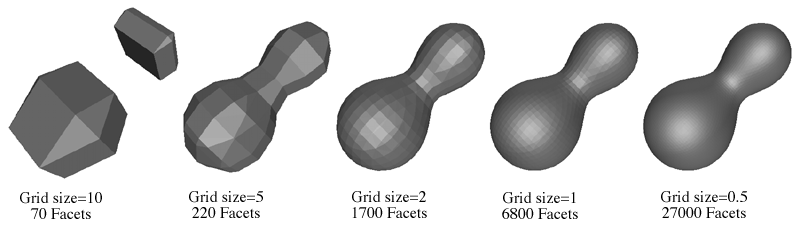
\includegraphics[width=\linewidth]{polygonise3.png}
  \caption{Marching cubes at different grid sizes \cite{bourke1994polygonising}}
  \label{fig:marching-cubes}
\end{figure}

The algorithm starts by dividing the space into a 3D grid, and samples the scalar field at the 8 corners of each cell. When an edge of a grid cell has one corner below \lstinline{isolevel} and one above, the edge intersects the isosurface, and we should generate a triangle there.
We can study all the possible configurations of edges intersecting the surfaces and determine that there are only 15 unique cases, for a total of 256 cases accounting flips and rotations.
Instead of computing on the spot the proper way to place the triangles in the cell, we pre-compute some lookup tables ahead of time. Usually, instead of computing the tables from scratch, people tend to copy the tables used in some foundational work or other projects. In our case we used the tables from Bourke's implementation \cite{bourke1994polygonising}. Note that there is no unique way to solve all the configurations, so any fixed table brings its own compromises or biases. There exist multi-pass approaches which attempt to mitigate this \cite{chernyaev1995marching}.

\begin{figure}[htbp]
  \centering
  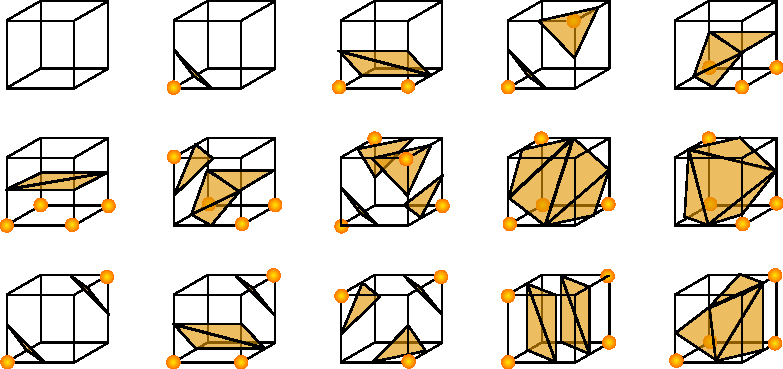
\includegraphics[width=1\linewidth]{unique-cases.pdf}
  \caption{15 unique cases of marching cubes \cite{wiki:mc_unique_cases}}
  \label{fig:unique-cases}
\end{figure}

We triangulate point clouds that are enclosed within a fixed room, and we want the generated geometry to be constrained by the room walls as well, while still being watertight. Moreover, if the room is not a multiple of the particle radius, some bordering cells will be clipped at the walls; we want the geometry to fill entirely these partial cells whenever required.

On each of these kernels, we use 3D block and grid dimensions, paired with a specialised \lstinline{cuda::std::mdspan} that we use to access more easily the 3D grid. We always launch a thread per ``work unit'': when computing the fields, we launch a thread per sampling point; when generating the triangles, one thread per grid cell.

A side note regarding the point's data type. All the algorithms implemented till now were generic and templated, however, marching cubes is not. Since we are implementing the algorithm in 3D, it would seem reasonable to use \lstinline{float3}, however, it is 12bytes long, thus a global memory read would require 3 separate load instructions, preventing memory coalescing. By ``wasting'' 4 bytes with \lstinline{float4} we get back coalescing with a performance bonus.
The fourth component can be used for operations preceding the triangulation (e.g. affine transformations). We provide a mapping kernel to convert from \lstinline{float3} to \lstinline{float4} applying a closure to each point. This way even if we receive the points as \lstinline{float3} (like in our demo) we pay the conversion price once and then stick to \lstinline{float4}.

When writing the output triangles we do so as a struct of three \lstinline{float3}, this is also inefficient. Unfortunately, this is the format used by the renderer and it's not reasonable to change it. We note that each thread writes a \emph{differently sized} batch of triangles sequentially to different memory locations; there isn't coalescing opportunity.

\enlargethispage{1\baselineskip}

\section{Computing scalar fields}

In theory (and in some classical applications) the field is computed from a mathematical function, ideally an actual density function. However, as in our case, it can also be estimated from a set of points, in a process called Kernel Density Estimation (KDE). A similar process is also used in statistics, to estimate the probability density function of a distribution, given a population.

The idea of KDE is to ``place'' a kernel density function centred at each point in the population, where the estimated density field is the sum of all the kernels, normalized if required. To sample a point, we just go over every point in the population and calculate how much it contributes, summing the value. Of course, such naive approach is prohibitively expensive.

With a spatial hash table we can restrict the iteration to the sampling point's neighbouring buckets. Since we are sampling exactly on the grid vertices, we set the cell size equal to the radius of the hashing function, so we only need to iterate over 8 buckets.

Now we need to choose an appropriate kernel. The naive choice would be the Gaussian bell, commonly used for KDE in statistics. However, the Gaussian never reaches 0, so we might lose contributions from outside the sampling volume, leading to potentially inconsistent values. The clipping shouldn't affect the result.

Other desirable properties are smoothness and continuity. The kernel should reach 0 smoothly and with a derivative of 0. The choice falls between ``poly6'' and ``Wendland $C^2$''; both designed for SPH and widely used in marching cubes. The first is cheap to compute, but its 0 gradient at the origin can cause artifacts. The second is more robust, though it requires the square root. We choose ``Wendland $C^2$'' because we are more likely to be limited by memory bandwidth rather than compute.

\begin{figure}[htbp]
  \centering
  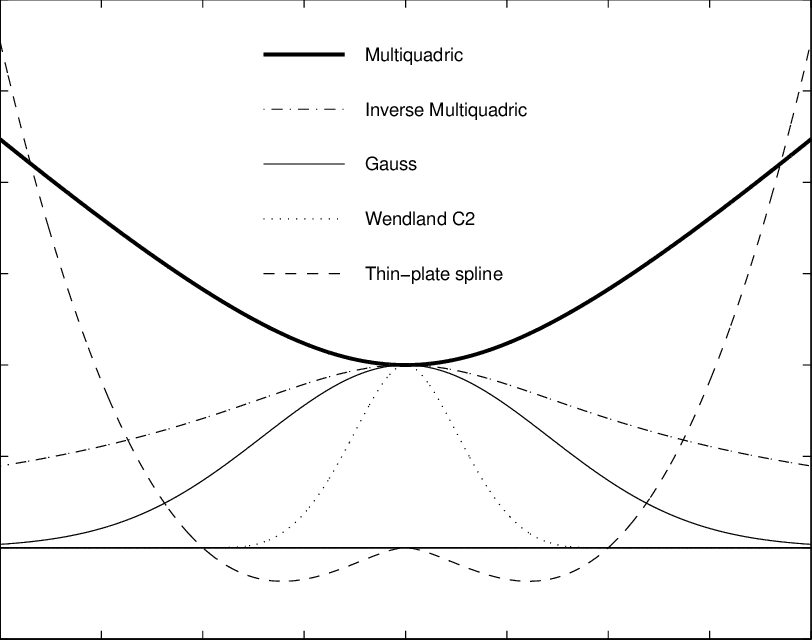
\includegraphics[width=\linewidth]{Some-radial-basis-functions.png}
  \caption{Some radial basis functions \cite{schaback2007practical}}
  \label{fig:some-rbfs}
\end{figure}

\begin{equation}
W(d) = 
\begin{cases} 
\sigma_3\left(1-\frac dr\right)^4\left(4\frac dr+1\right)&\text{if }0\leq d<r\\
0&\text{otherwise}
\end{cases}
\end{equation}

Where the dimensional normalisation factor $\sigma_3$ is ignored, losing the mass\slash density conservation property not required by our application. $r$ is the particle radius and $d$ is the euclidean distance between the two points.

\newpage

\begin{lstlisting}[caption={Wendland $C^2$ kernel density function}, language=c++]
// estimate *unnormalised* Wendland C2 density
GPU float calculate_density(Params const params, float3 const sample_point, float3 const point) {
  float const dist_sq = sq_dist(sample_point, point);

  if (dist_sq >= params.particle_radius_sq) {
    return 0.0f;
  }

  // fast sqrt: sqrt(x) == x * rsqrt(x). +epsilon guards against
  // rsqrtf(0) -> inf -> 0*inf -> NaN when node_pos == point_pos exactly
  float const distance = dist_sq * rsqrtf(dist_sq + cuda::std::numeric_limits<float>::min());

  // Wendland C2 kernel
  float const u = distance / params.particle_radius;
  float const term = 1.0f - u;
  float const w = (term * term * term * term) * (4.0f * u + 1.0f);
  return w;
}
\end{lstlisting}

The geometry cut-off effect is achieved with a mix of techniques we'll discuss in a later section. In this kernel the sample point is clamped to the room boundary before sampling, and its position dictates which buckets we need to inspect. This is handled by the \lstinline{get_neighbourhood_bounds} function.

\begin{itemize}
  \item If one of the coordinates is 0 (lower room boundaries), the sample point is still aligned to the grid. We just skip the buckets outside the room
  \item If one coordinate sits at the upper room boundary, the clamping misaligns it with the grid. To compensate, we check one extra cell layer inward in each clamped dimension. We still skip the buckets outside the room, ensuring we never iterate over more than 8 buckets 
\end{itemize}

If a point on the boundary is above \lstinline{isolevel}, we clamp it at exactly \lstinline{isolevel}.

Because our hash function can clash, we need to make sure to not iterate over the same bucket twice. We store the seen hashes in a local array, through a switch-case writing function to prevent local memory spilling. The array is small enough to justify avoiding the shared memory.

\begin{lstlisting}[caption={Compute scalar fields}, language=c++]
template <is_hasher<u323> Hasher>
KERNEL void compute_scalar_fields(float4 const *const points,
                                  HashTable const *const table,
                                  Params const params,
                                  float *const linearized_fields,
                                  Hasher const hasher) {
  using Key = Key<float4, Hasher>;
  u323span const fields(linearized_fields, extents_3d{params.samples.x, params.samples.y, params.samples.z});
  u323 const coords = (vec_cast<u323>(blockIdx) ^ vec_cast<u323>(blockDim)) + vec_cast<u323>(threadIdx);

  if (is_out_of_bounds(coords, params.samples))
    return;
(*@\newpage@*)
  // convert index to float at maximum precision
  auto const grid_point = get_grid_point(coords, params.particle_radius);
  float3 const sample_point = clamp_point(grid_point, params.room);

  float field = 0.0f;
  typename Key::KeyType seen_hashes[8];
  u8 seen_count = 0;

  auto const [starts, bounds] = get_neighbourhood_bounds(coords, params.samples);
  for (u83 ind = {}; ind.z < 2; ++ind.z) {
    for (ind.y = 0; ind.y < 2; ++ind.y) {
      for (ind.x = 0; ind.x < 2; ++ind.x) {
        // this style of iterations keeps seen_hashes[] in the registers
        if (!(ind < bounds)) {
          continue;
        }

        s83 const offsets = starts + ind;
        typename Key::KeyType const hash = hasher(coords + offsets);
        // check for clashes in previous hashes
        if (find(seen_hashes, seen_count, hash) < seen_count) {
          continue;
        }
        // keep seen_hashes[] in the registers
        add_checked_hash(seen_hashes, seen_count, hash);

        if (auto const bucket = table->lookup(hash); bucket) {
          for (u32 i = bucket->begin; i < bucket->end; ++i) {
            float3 const point = project4to3(points[i]);
            // currently calculated using Wendland C2
            field += calculate_density(params, sample_point, point);
          }
        }
      }
    }
  }

  field = is_out_of_bounds(grid_point, params.room) ? fminf(field, params.isolevel) : field;
  fields[coords] = field;
}
\end{lstlisting}

\section{Generating triangles}

To access the lookup tables, we simply check which corners of the cell are below \lstinline{isolevel} and flag them on an 8bit bitmask, which acts as an index. Note that the tables and the \emph{order} of the bits in the mask must be coherent. Interestingly, flipping the bits flips the generated triangles, keeping the same shape.

\newpage

\subsection{Triangle counting}

Before generating the triangles we must allocate an array to store them, as well as determining the position where each thread will be writing. We first create an array with one cell per thread, then, we launch a kernel to populate it. We use a precomputed helper table that maps each case to the number of triangles it generates. Then we compute the prefix sum of this array, using the standalone prefix sum algorithm.
We add the usual extra cell at the end to obtain the total number of triangles, the length of the triangle buffer.

\begin{lstlisting}[caption={Count how many triangles will be generated}, language=c++]
KERNEL void
count_triangles(Params const params, float const *const linearized_fields, u32 *const linearized_triangle_counts) {
  u323span const fields(linearized_fields, extents_3d{params.samples.x, params.samples.y, params.samples.z});
  u323span const triangle_counts(linearized_triangle_counts,
                                 extents_3d{params.cells.x, params.cells.y, params.cells.z});
  u323 const coords = (vec_cast<u323>(blockIdx) ^ vec_cast<u323>(blockDim)) + vec_cast<u323>(threadIdx);

  if (is_out_of_bounds(coords, params.cells))
    return;

  if (coords == u323{}) {
    // thread 0 writes 0 on an extra cell of triangle counts
    // after the prefix_sum the cell will hold the total number of triangles
    // this allows to store the prefixes on the same buffer as the counts
    linearized_triangle_counts[params.cell_count()] = 0;
  }

  u8 case_index = 0;
  for (u8 i = 0; i < 8; ++i) {
    // read the corner of the cell
    u323 const corner = coords + get_cell_corner_offsets(i);
    // build the corner bitmask (1 means outside the object)
    case_index |= static_cast<u8>(fields[corner] <= params.isolevel) << i;
  }

  triangle_counts[coords] = triangle_table.counts[case_index];
}
\end{lstlisting}

\subsection{Triangle generation}

In the lookup table, triangles are represented as a list of cell edges. We number them from 0 to 11. The table contains 0 to 5 triples of these indices for each case.

Now, we could simply connect edges by their middle point, but that would produce a ``blocky'' geometry. We can instead make use of the density field value by interpolating where the isosurface should be, giving us a result much more representative of the data.

\newpage

The intuition is that if an edge vertex's field is just below/above \lstinline{isolevel}, it means that it's just outside/inside of the isosurface, thus the triangle's vertex should be closer to it. Conversely, if the field value is far from \lstinline{isolevel}, the triangle's vertex should be further away as well.

\begin{equation}
p_1+\frac{\varphi-f_1}{f_2-f_1}(p_2-p_1)
=(1-\frac{\varphi-f_1}{f_2-f_1})p_1+\frac{\varphi-f_1}{f_2-f_1}p_2
\end{equation}

For numerical stability, the function includes a fallback when the field values are too close: we simply return the middle point of the edge.

\begin{lstlisting}[caption={Interpolate triangle vertex on an edge}, language=c++]
float3 get_edge_vertex(Params const &params, u8 const edge, u323 const cell, SampleData const (&data)[8]) {
  auto const [i1, i2] = get_edge_indices(edge);
  float3 const corner1 =
      clamp_point(get_grid_point(cell + get_cell_corner_offsets(i1), params.particle_radius), params.room);
  float3 const corner2 =
      clamp_point(get_grid_point(cell + get_cell_corner_offsets(i2), params.particle_radius), params.room);
  SampleData data1 = get_corner_data(data, i1);
  SampleData data2 = get_corner_data(data, i2);

  float const scale = fmaxf(fabsf(data1.field), fmaxf(fabsf(data2.field), fabsf(params.isolevel)));
  float const tolerance = 8.f * cuda::std::numeric_limits<float>::epsilon() * fmaxf(scale, 1.0f);
  float const coefficient = fabsf(data1.field - data2.field) <= tolerance
                                ? 0.5f
                                : (params.isolevel - data1.field) / (data2.field - data1.field);
  return interpolate(corner1, corner2, coefficient);
}
\end{lstlisting}

Like the previous kernel, \lstinline{data} is accessed through a switch-case helper function \lstinline{get_corner_data} to prevent local memory spillage.
\lstinline{get_cell_corner_offsets} and \lstinline{get_edge_indices} are usually implemented as tables; we have synthesized them as procedural bitwise operations to avoid unnecessary memory accesses.

The same clamping to the room boundary applies when interpolating.

\begin{lstlisting}[caption={Compute triangles}, language=c++]
KERNEL void make_triangles(Params const params,
                           float const *const linearized_fields,
                           u32 const *const linearized_triangle_prefixes,
                           float33 *const triangles,
                           float33 *const normals) {

  //////// Omitted ////////

  SampleData sample_data[8];
  u8 case_index = 0;
  for (u8 i = 0; i < 8; ++i) {
    sample_data[i].field = fields(corner.x, corner.y, corner.z);
    case_index |= static_cast<u8>(sample_data[i].field <= params.isolevel) << i;
  }

  u8 const triangle_count = triangle_table.counts[case_index];
  if (triangle_count == 0)
    return;

  u32 const start = triangle_prefixes[coord];
  for (u8 i = 0; i < triangle_count; ++i) {
    auto const p1 =
        get_edge_vertex(params, triangle_table.triangles[case_index][i][0], coord, sample_data);
    auto const p2 =
        get_edge_vertex(params, triangle_table.triangles[case_index][i][1], coord, sample_data);
    auto const p3 =
        get_edge_vertex(params, triangle_table.triangles[case_index][i][2], coord, sample_data);

    triangles[start + i] = {
        {p1, p2, p3}
    };
  }
}
\end{lstlisting}

It is paramount for every iteration, bitmask and table to be coherent. In our case we used the tables from Bourke's implementation \cite{bourke1994polygonising}, so we built the rest of the logic around that.
Note that also the vertex order (winding) becomes meaningful when rendering, as it determines the triangle's facing direction. This is especially true in the case of real-time renderers.

\section{Room cut-off effect}

Without intervention, with the standard marching cubes algorithm we might observe two issues:

\begin{enumerate}
  \item Some triangles are generated beyond the room boundaries.
  
  This happens when the room is not a multiple of the particle radius, because the outermost grid cells are not perfectly aligned with the room walls
  \item The geometry is not closed along the room walls.
  
  This happens when enough points cluster near the outermost sampling points, inducing a field value above \lstinline{isolevel}. The algorithm sees it as inside the isosurface, so it leaves the mesh open, expecting a further cell to close it.
\end{enumerate}

Our first approach was to iterate over a ``sarcophagus of virtual cells'' enclosing the room, clamping the triangle vertices to plug the holes. This seemed to work, but it was incorrect: a cell geometry can overlap if squished, producing artifacts and degenerate triangles along the edges of the room. This approach requires a proper mesh clipping algorithm, far too expensive and complex to implement.

We found an alternative solution that retains most of the cut-off look we wanted, with little to no additional cost or complexity.

Firstly we prevent the boundary fields to be above \lstinline{isolevel}, forcing the algorithm to close the geometry. Point outside the geometry retain their field value, keeping the geometry true to the data. Points inside will be considered barely outside, forcing the interpolation to generate the triangles flush to the room walls.

Next, we intervene on the generation phase. Instead of clamping the interpolated result, we clamp the interpolation points. This keeps the geometry inside the room while preserving the interpolation ratios. Note that both sample and interpolation points are clamped so they refer to the same location. 

All this together gives us a geometry that neatly fills the room, without holes or protrusions, whilst remaining true to the data.

\section{Normals computation}

In computer graphics, a ``normal'' is an unit vector perpendicular to a facet. The renderer uses them to calculate the colour of a fragment, by measuring how the normal aligns with the light source. Normals can add information to a mesh allowing for a more accurate shading.

Given a vertex, we can use the cross product to compute the normal of each adjacent triangle and then store the average, obtaining a smooth look. The shading pipeline can then interpolate a normal for each point of the surface in a process called Phong shading \cite{Bui1975IlluminationFC}. Unfortunately, this approach is not viable in a marching cube context because each triangle has its own independent vertices and there's no data structure to query adjacencies.

\begin{figure}[htbp]
  \centering
  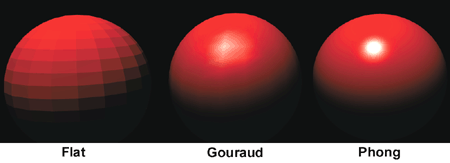
\includegraphics[scale=1]{flat-gouraud-phong.png}
  \caption{Phong compared to other shading models \cite{salvatierra2015openglshading}}
  \label{fig:shading-models}
\end{figure}

Fortunately, the scalar field is a much better basis for computing normals, because it's directly tied to the data we are actually trying to represent. The mathematical tool we use is the gradient of the scalar field:

\begin{equation}
\nabla f(p)=\begin{bmatrix}
\frac{\partial f}{\partial x}(p)\\[1ex]
\frac{\partial f}{\partial y}(p)\\[1ex]
\frac{\partial f}{\partial z}(p)
\end{bmatrix}
\end{equation}

\newpage

The gradients form a vector field that points in the direction of maximum density increase at any given coordinate. By definition, the isovalue $\varphi$ is constant along the isosurface, thus given a small tangent vector $v_t$, we have:

\begin{equation}
\nabla f\cdot v_t=0
\end{equation}

Meaning the gradient is always perpendicular, pointing inward. If we compute $\nabla f$ at each sampling point, we can interpolate it together with the triangles' vertices. Then the normal is simply the normalized, inverted gradient.

We store the gradient and the field value inside the \lstinline{SampleData} struct.

\begin{lstlisting}[caption={Gradient interpolation}, language=c++]
GPU pair<float3, float3>
get_edge_vertex(Params const &params, u8 const edge, u323 const cell, SampleData const (&data)[8]) {

  //////// Omitted ////////
  
  float3 const avg_gradient = interpolate(data1.gradient, data2.gradient, coefficient);
  float const sq_avg_gradient = avg_gradient * avg_gradient;
  return {interpolate(corner1, corner2, coefficient),
          ((sq_avg_gradient > 0.f) ? avg_gradient * -rsqrtf(sq_avg_gradient) : float3{})};
}
\end{lstlisting}

At the end of the kernel, we store the normals in a separate output array with the same length as the triangle array. They are accessed as two separate arrays because that is what the renderer expects, but we make a single allocation.


\begin{lstlisting}[caption={Compute triangles with normals}, language=c++]
KERNEL void make_triangles(Params const params,
                           float const *const linearized_fields,
                           u32 const *const linearized_triangle_prefixes,
                           float33 *const triangles,
                           float33 *const normals) {

  //////// Omitted ////////

  u32 const start = triangle_prefixes[coord];
  for (u8 i = 0; i < triangle_count; ++i) {
    auto const [p1, gradient1] =
        get_edge_vertex(params, triangle_table.triangles[case_index][i][0], coord, sample_data);
    auto const [p2, gradient2] =
        get_edge_vertex(params, triangle_table.triangles[case_index][i][1], coord, sample_data);
    auto const [p3, gradient3] =
        get_edge_vertex(params, triangle_table.triangles[case_index][i][2], coord, sample_data);
    float3 const fallback_normal = cross(p2 - p1, p3 - p1);

    triangles[start + i] = {
        {p1, p2, p3}
    };(*@\newpage@*)
    normals[start + i] = {is_valid_normal(gradient1) ? gradient1 : fallback_normal,
                          is_valid_normal(gradient2) ? gradient2 : fallback_normal,
                          is_valid_normal(gradient3) ? gradient3 : fallback_normal};
  }
}
\end{lstlisting}

We can compute the scalar field’s gradient in two ways: analytically or through a grid-based approach. While the analytical method is more mathematically elegant, the grid-based approach proved more robust for our kind of data.

\subsection{Analytical gradients}

Since differentiation is linear, we can compute the gradient on a term-by-term basis. We sum the contribution of each neighbouring point $p_i$, as we already do for each sample point:

$$
\nabla(f_{p_1}+f_{p_2}+\dots)
=\nabla f_{p_1}+\nabla f_{p_2}+\dots
$$

We first derive the Wendland $C^2$ function using the chain rule:

\begin{equation}
\begin{aligned}
& W(d)=\left(1-\frac dr\right)^4\left(4\frac dr+1\right)\\
& =(1-u)^4(4u+1) & \left[u=\frac dr\right]\\
& \frac{\mathrm{d}W}{\mathrm{d}u}=4(1-u)^4-4(4u+1)(1-u)^3\\
& 4(1-u)^3(1-u-4u-1)\\
& -20u(1-u)^3
\end{aligned}
\end{equation}

\begin{equation}
\frac{\mathrm{d}u}{\mathrm{d}d}=\frac 1r
\end{equation}

\begin{equation}
\frac{\mathrm{d}W}{\mathrm{d}d}=-20\frac d{r^2}\left(1-\frac dr\right)^3
\end{equation}

Then we scale an unit vector which encodes the contribution's direction:

\begin{align}
& \vec d_i=x-p_i & \left[\text{where $x$ is the sample point}\right]\\
& \nabla f_{p_i}=\frac{\mathrm{d}W}{\mathrm{d}d_i}\frac{\vec d_i}{d_i}=-\frac{20}{r^2}\left(1-\frac {d_i}r\right)^3\vec d_i & \left[\text{since }d_i=\|\vec d_i\|\right]
\end{align}

\advance\voffset by -1\baselineskip 
\enlargethispage{2\baselineskip}
\addtolength{\footskip}{1\baselineskip}

This approach allows us to elegantly compute the gradient along with the field value. However, it doesn't guarantee results coherent with the final marching cubes mesh. Intuitively, this calculation is sensitive to the direction of each neighbouring point, whereas the triangulation algorithm only sees density as a scalar value. This brought rendering artifacts visible in \cref{fig:analytical-normals} and we had to change approach.

\clearpage
\advance\voffset by 1\baselineskip 
\addtolength{\footskip}{-1\baselineskip}

\begin{figure}[htbp]
  \centering
  \includesvg[scale=0.3]{gradient-flipping.svg}
  \caption{The gradient at the sampling points (direction of the triangles) can point outside of the isosurface for points under the surface (in red). This can result in the interpolated gradients (in purple) pointing out of the isosurface.}
  \label{fig:gradient-flipping}
\end{figure}

\subsection{Central difference gradients}

This method approximates the derivative by simply looking at the change in field values across adjacent grid vertices.

\begin{equation}
\begin{bmatrix}
\frac{\partial f}{\partial x}(p)\\[1ex]
\frac{\partial f}{\partial y}(p)\\[1ex]
\frac{\partial f}{\partial z}(p)
\end{bmatrix}
\approx
\frac 1{2r}
\begin{bmatrix}
f_{x+1,y,z}-f_{x-1,y,z}\\
f_{x,y+1,z}-f_{x,y-1,z}\\
f_{x,y,z+1}-f_{x,y,z-1}
\end{bmatrix}
\end{equation}

In the code we ignore the $\frac 1{2r}$ factor because the gradient is later normalized anyway.

The downside is that this approach is susceptible to normal cancellation. This is especially true on boundaries where the field value saturates to \lstinline{isolevel}. In this case we cant normalize a 0 vector, so we fallback to the triangle normal.

\enlargethispage{1.1\baselineskip}

\begin{lstlisting}[caption={Compute triangles with normals}, language=c++]
KERNEL void make_triangles(Params const params,
                           float const *const linearized_fields,
                           u32 const *const linearized_triangle_prefixes,
                           float33 *const triangles,
                           float33 *const normals) {
  
  //////// Omitted ////////

  SampleData sample_data[8];
  u8 case_index = 0;
  for (u8 i = 0; i < 8; ++i) {
    u323 const corner = coord + get_cell_corner_offsets(i);
    sample_data[i].field = fields(corner.x, corner.y, corner.z);
    case_index |= static_cast<u8>(sample_data[i].field <= params.isolevel) << i;
  }
  u8 const triangle_count = triangle_table.counts[case_index];
  if (triangle_count == 0)
    return;

  for (u8 i = 0; i < 8; ++i) {
    u323 const corner = coord + get_cell_corner_offsets(i);
    float3 const f_next = {
        (corner.x + 1 < params.samples.x) ? fields(corner.x + 1, corner.y, corner.z) : params.isolevel,
        (corner.y + 1 < params.samples.y) ? fields(corner.x, corner.y + 1, corner.z) : params.isolevel,
        (corner.z + 1 < params.samples.z) ? fields(corner.x, corner.y, corner.z + 1) : params.isolevel};
    float3 const f_prev = {
        (corner.x > 0) ? fields(corner.x - 1, corner.y, corner.z) : params.isolevel,
        (corner.y > 0) ? fields(corner.x, corner.y - 1, corner.z) : params.isolevel,
        (corner.z > 0) ? fields(corner.x, corner.y, corner.z - 1) : params.isolevel,
    };
    sample_data[i].gradient = f_next - f_prev;
  }
  
  //////// Omitted ////////
}
\end{lstlisting}

\begin{figure}[htbp]
  \centering
  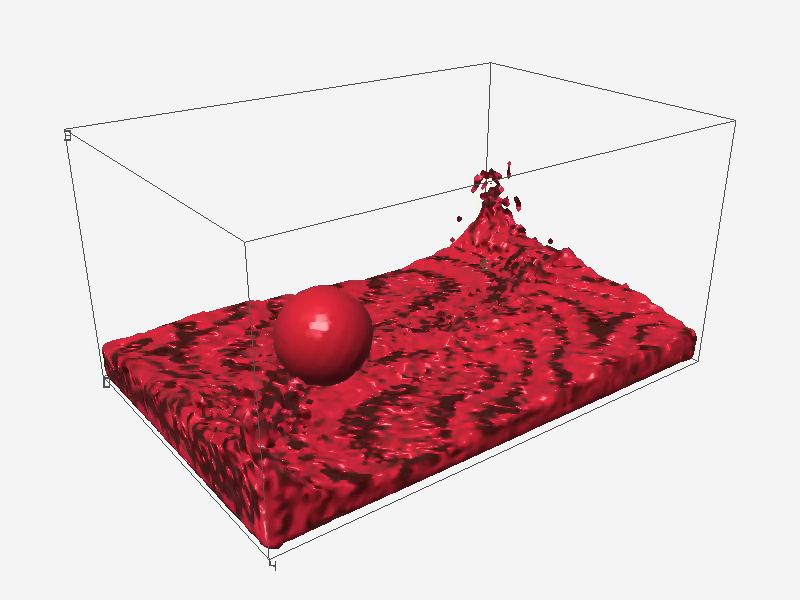
\includegraphics[width=\linewidth]{analytical-normals.png}
  \caption{Rendering with analytical normals}
  \label{fig:analytical-normals}
\end{figure}

\begin{figure}[htbp]
  \centering
  \includesvg[scale=0.2]{scalar-field-cancellation.svg}
  \caption{Two sampling points (dotted) with gradient 0, a vertex interpolated between the two will have normal 0, causing division-by-zero errors. The triangles contribute to the gradient on the left, and the squares to the gradient on the right. Same colour means same field value.}
  \label{fig:field-cancellation}
\end{figure}

\begin{figure}[htbp]
  \centering
  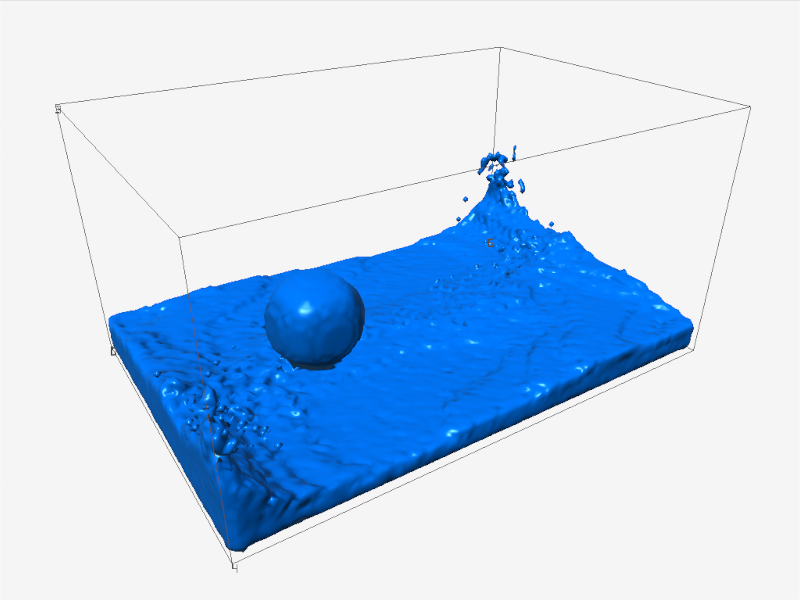
\includegraphics[width=1\linewidth]{grid-normals-o.png}
  \caption{Rendering with grid based normals. Using grid-based normals introduces visible grid steps across the sphere.}
  \label{fig:grid-normals}
\end{figure}

\chapter{Streaming from disk to device memory}

Since this cube marcher implementation if fast enough for a real-time application, the demo features a ``player'' mode that loads point cloud recordings, triangularizing them on the fly. At 60 frames per second and millions of points per frame, these recording files can overwhelm both device and host memory, hence we require some streaming producer-consumer technique. We upload the frames into device memory while they are being triangularized, in a double buffered way: while one buffer is being triangulated and rendered, the other is being copied to, and vice versa. Ultimately need to deal with two challenges: move the data from disk to host memory, and then from host memory to the device.

The file format begins with a header containing the room size, the number of points in each frame (constant for all frames) and the total number of frames.

\section{Memory mapping}

Instead of manually reading from disk the individual frames (with massive overhead) we map the file in ram. This allows us to avoid explicitly reading from disk, and let the operating system exploit every advanced algorithm and heuristic that already powers memory swapping. If the file is small enough to fit in ram, the OS will upload it in host memory entirely, and if it isn't the OS will try to minimize the latency.

Because Windows and Linux have different APIs we wrote a simpler C interface, implemented with conditional compilation.

This method has great advantages but introduces a major weakness: the memory is paged, and therefore incompatible with \lstinline{cudaMemcpyAsync} (which requires page-locked memory). This is unavoidable, as paging is exactly the mechanism performing the streaming.

\begin{lstlisting}[caption={Memory mapping interface}, language=c]
typedef struct MappedFile {
  void const *map_ptr;
  void const *data;
  size_t map_size;
  size_t size;
} MappedFile;

MmapError mmap_file(FILE *file, size_t offset, size_t size, MappedFile *out_mapping);
void munmap_file(MappedFile *mapping);
\end{lstlisting}

\section{Streaming with double buffering}

We cannot use \lstinline{cudaMemcpyAsync} to upload the frames to device memory, but double buffering only makes sense if the work on the two buffers happens in parallel. We need to implement asynchronicity manually.

The idea is to run the synchronous \lstinline{cudaMemcpy} (which does not require page locking) on a worker thread, allowing the main thread to continue issuing kernels and other CUDA commands while the copy is taking place. We use two preallocated buffers: the worker thread waits for buffer 0 to be released, writes to it, and signals the main thread that it's ready; it then switches to buffer 1, waits for it to be released, and so on. Meanwhile the main thread waits for buffer 0 to be ready, uses it, releases it, renders, and switches to buffer 1.

Ideally, both threads should be able to use the buffers as soon as they are released, regardless of the other's status; moreover, the main thread should be able to schedule kernels and delegate waiting to the GPU. A basic barrier is insufficient because it forces a symmetric synchronization pattern (lockstep). A queue-like solution, however, allows the worker thread to preload both buffers in scenarios where the main thread has released its buffer but is still computing.

The obvious choice to synchronize the two threads would be stream events. Unfortunately, stream events are not suited for mixed synchronous and asynchronous code: each \lstinline{cudaStreamWaitEvent} only waits for the \lstinline{cudaEventRecord}s that have already been scheduled. With async code, it's possible to schedule a stream that records an event, \emph{followed by} a stream that awaits it, and this would work as expected. However with synchronous code, the worker can't issue \lstinline{cudaEventRecord} until it has completed the \lstinline{cudaMemcpy}. If the main thread awaits on the event too early, it just skips waiting and proceeds. This issue manifests in both directions, as the main thread must copy data back from the GPU synchronously.

The solution is two lower level commands: \lstinline{cuStreamWaitValue32} to block the command queue and wait for a device-accessible location to read a certain value, and \lstinline{cuStreamWriteValue32} to issue a write in a device-accessible location. With these primitives we can schedule both wait and release operations on the main thread.
Unfortunately we can't use them on the worker thread as well, because the \lstinline{cuStreamWaitValue32} command blocks the command queue entirely. If the release is scheduled on the same queue, it will never execute and cause a deadlock. Not only there is no reliable way to guarantee that the two streams will schedule commands on different queues; but they are \emph{expected} to use the same one.
This is because these APIs are meant to pair with contexts that bypass the command queues, such as Vulkan/DirectX interop, or (in our case) direct device-mapped memory access. For this reason, the worker thread performs regular reads and writes on device-mapped memory, utilizing atomic operations just to force memory orderings.

\begin{lstlisting}[caption={Worker thread loop}, language=c]
static int worker_loop(void *const arg) {
  Streamer const *const streamer = (Streamer const *)arg;
  u8 slot = 0;
  u32 seq = 0;(*@\newpage@*)
  for (u32 frame = 0; !atomic_load(&streamer->stop_requested);
       frame = (frame + streamer->frameskip + 1) % streamer->total_frames, // choose next frame
       seq += slot,                                                        // increment every two iterations
       slot = 1 - slot                                                     // flip slot
  ) {

    // spin wait for gpu_done
    while (atomic_load_explicit(streamer->gpu_done[slot], memory_order_acquire) < seq &&
           !atomic_load(&streamer->stop_requested)) {
      thrd_yield();
    }

    if (atomic_load_explicit(&streamer->stop_requested, memory_order_acquire))
      return 0;

    // synchronoud copy
    TRAP_CUDAPI(cudaMemcpy(streamer->buffers[slot],
                           &((float3 const *)streamer->mapped_file.data)[(u64)streamer->num_particles * (u64)frame],
                           streamer->frame_size, cudaMemcpyHostToDevice),
                "streamer: worker thread upload frame");

    // publish upload_done
    atomic_store_explicit(streamer->upload_done[slot], seq + 1, memory_order_release);
  }
  return 0;
}
\end{lstlisting}

\enlargethispage{2\baselineskip}

\begin{lstlisting}[caption={Release and aquire functions for the main thread}, language=c]
// acquire: make the compute stream wait for the upload
float3 *
streamer_acquire_next_frame(Streamer const *const streamer, u32 const buf_idx, cudaStream_t const compute_stream) {
  u32 const wait_val = streamer->consumer_seq[buf_idx];

  handle_cuda_driver_error(
      cuStreamWaitValue32(compute_stream, streamer->upload_done_dptr[buf_idx], wait_val, CU_STREAM_WAIT_VALUE_GEQ),
      "streamer: wait to aquire frame");

  return streamer->buffers[buf_idx];
}

// release: tell the worker the buffer is free
void streamer_release_frame(Streamer *const streamer, u32 const buf_idx, cudaStream_t const compute_stream) {
  u32 const seq = streamer->consumer_seq[buf_idx];

  handle_cuda_driver_error(
      cuStreamWriteValue32(compute_stream, streamer->gpu_done_dptr[buf_idx], seq, CU_STREAM_WRITE_VALUE_DEFAULT),
      "streamer: release frame");

  ++streamer->consumer_seq[buf_idx];
}
\end{lstlisting}

\chapter{Demo}

To demonstrate our implementations we wrote a small C program with three modes:

\begin{description}
    \item[test] runs and verifies each of the algorithms on a random point cloud
    \item[random] triangulates and renders a random point cloud
    \item[player] plays a 3D animation as a sequence of triangulated point clouds
\end{description}

We use \lstinline{raylib} \cite{raylib} to provide a simple interactive viewer which can modify grid cell size and \lstinline{isolevel} on the fly.

Technically, since both the triangulation and rendering run on the GPU, the algorithm could write directly to an OpenGL buffer. This however requires a lot of complex boilerplate code with dubious performance gains. We deemed it out of scope and opted to copy each frame to host memory before rendering. Interestingly, this allows for the rendering and triangulation to run on separate GPUs (on some machines).

We also allocate and free every buffer used by the algorithm each time it is called (with the exception of the input buffer). A more efficient approach would be allocating the buffers (of known size) once and reuse them at each invocation. However this implementation is more involved and requires more device memory. We have observed that on smaller GPUs, we can run out of memory before saturating the computing power; therefore, we opted to keep this ``stateless'' API to minimize memory pressure.

\section{Test}

This mode generates a random point cloud of the length and size specified. Then it runs each of the algorithms and verifies the result.

The sort is verified by downloading the sorted array from device memory and verifying the hashes are ordered. The standalone prefix sum is verified by comparing the result to a CPU scan. The hash table is verified using a validating kernel.

The marching cubes algorithm is not verified automatically, but if the number of triangles is small enough, they are printed for manual verification.

\section{Player}

This mode is intended to demonstrate the effectiveness of the marching cube algorithm. We stream point cloud animations from a recording file with the techniques explained before. We also provide a python script to generate these files with the SPlisHSPlasH \cite{SPlisHSPlasH_Library} SPH solver.

Because the file is generated ahead of time, we can use high precision simulation algorithms that could never run in real-time. The algorithm can generate detailed geometries from dense clouds, showcasing how it can be tuned to preserve detail.

\section{Random}

This is the mode intended to stress the compute by minimizing I/O. We simply generate a set of random points directly in the GPU, triangulate and render. The triangulation is always ran at every frame to showcase the real-time capabilities of the implementation. It's also possible to regenerate the random points automatically every \lstinline{k} frames.

\bibliographystyle{alpha}
\bibliography{bibliography}
\addcontentsline{toc}{chapter}{Bibliography}

\end{document}
